\documentclass[review]{elsarticle}
 
\usepackage{lineno,hyperref}
\modulolinenumbers[5]

\journal{Journal of \LaTeX\ Templates}

%%%%%%%%%%%%%%%%%%%%%%%
%% Elsevier bibliography styles
%%%%%%%%%%%%%%%%%%%%%%%
%% To change the style, put a % in front of the second line of the current style and
%% remove the % from the second line of the style you would like to use.
%%%%%%%%%%%%%%%%%%%%%%%

%% Numbered
%\bibliographystyle{model1-num-names}

%% Numbered without titles
%\bibliographystyle{model1a-num-names}

%% Harvard
%\bibliographystyle{model2-names.bst}\biboptions{authoryear}

%% Vancouver numbered
%\usepackage{numcompress}\bibliographystyle{model3-num-names}

%% Vancouver name/year
\usepackage{numcompress}\bibliographystyle{model4-names}\biboptions{authoryear}

%% APA style
%\bibliographystyle{model5-names}\biboptions{authoryear}

%% AMA style
%\usepackage{numcompress}\bibliographystyle{model6-num-names}

%% `Elsevier LaTeX' style
%\bibliographystyle{elsarticle-num}
%%%%%%%%%%%%%%%%%%%%%%%
\usepackage{xeCJK}
\usepackage{bm}
\usepackage{amsmath}
\usepackage{amssymb}
\usepackage{amsthm}
\usepackage{graphicx}
\usepackage{color}
\usepackage{booktabs}

\DeclareMathOperator{\mytr}{tr}
\DeclareMathOperator{\mydiag}{diag}
\DeclareMathOperator{\myrank}{Rank}
\DeclareMathOperator{\myE}{E}
\DeclareMathOperator{\myVar}{Var}





\theoremstyle{plain}
\newtheorem{theorem}{\quad\quad Theorem}
\newtheorem{proposition}{\quad\quad Proposition}
\newtheorem{corollary}{\quad\quad Corollary}
\newtheorem{lemma}{\quad\quad Lemma}
\newtheorem{example}{Example}
\newtheorem{assumption}{\quad\quad Assumption}
\newtheorem{condition}{\quad\quad Condition}

\theoremstyle{definition}
\newtheorem{remark}{\quad\quad Remark}
\theoremstyle{remark}
\begin{document}

\begin{frontmatter}

\title{High-dimensional two-sample test under spiked covariance}

%% Group authors per affiliation:
    \author[mymainaddress]{Rui Wang}
    \author[mymainaddress,mysecondaryaddress]{Xingzhong Xu\corref{mycorrespondingauthor}}
\cortext[mycorrespondingauthor]{Corresponding author}
\ead{xuxz@bit.edu.cn}
    \address[mymainaddress]{School of Mathematics and Statistics, Beijing Institute of Technology, Beijing 
    100081,China}
    \address[mysecondaryaddress]{Beijing Key Laboratory on MCAACI, Beijing Institute of Technology, Beijing 100081,China}
%\fntext[myfootnote]{Since 1880.}

%% or include affiliations in footnotes:
%\author[mymainaddress,mysecondaryaddress]{Elsevier Inc}
%\ead[url]{www.elsevier.com}



\begin{abstract}
    This paper considers testing the means of two $p$-variate normal samples in high dimensional setting.  The covariance matrices are assumed to be spiked, which often arises in practice. 
    We propose a new test procedure through projection on the orthogonal complement of principal space.
    The asymptotic normality of the new test statistic is proved and the power function of the test is given.
    Theoretical and simulation results show that the new test outperforms existing methods substantially when the covariance matrices are spiked. Even when the covariance matrices are not spiked, the new test is acceptable.
\end{abstract}

\begin{keyword}
    high dimension, mean test, orthogonal complement of principal space, spiked covariance
\end{keyword}

\end{frontmatter}

%\linenumbers



\section{Introduction}

Suppose that $X_{k,1},\ldots,X_{k,n_k}$  are independent identically distributed (i.i.d.) as $N_p(\mu_k,\Sigma)$, where $\mu_k$ and $\Sigma$ are unknown, $k=1,2$. We consider the hypothesis testing problem:

\begin{equation}\label{problem}
    H_0:\mu_1=\mu_2\quad \textrm{vs.}\quad H_1:\mu_1\neq \mu_2.
\end{equation}
 In this paper, high dimensional setting is adopted, i.e., the dimension $p$ varies as $n$ increase, where $n=n_1+n_2$ is the total sample size.
Testing hypotheses~\eqref{problem} is important in many applications, including biology, finance and economics.
Quite often,  these data have strong correlations between variables.
When strong correlations exist, covariance matrices are often spiked in the sense that a few eigenvalues are distinctively larger than the others.
This paper is devoted to
testing hypotheses~\eqref{problem} in high dimensional setting with spiked covariance.


A classical test for hypotheses~\eqref{problem} is Hotelling's $T^2$ test.
Hotelling's test statistic is ${(\bar{X}_1-\bar{X}_2)}^T S^{-1}(\bar{X}_1-\bar{X}_2)$, where
    $
    S=
{(n-2)}^{-1}\sum_{k=1}^2\sum_{i=1}^{n_k} (X_{k,i}-\bar{X}_k) {(X_{k,i}-\bar{X}_k)}^T
    %{(n-2)}^{-1}((n_1-1)S_1+(n_2-1)S_2)
    $
is the pooled sample covariance matrix.
However, Hotelling's test is not defined when $p\geq n-1$.
Moreover,~\cite{Bai1996Efiect} showed that even if $p<n-1$, Hotelling's test suffers from low power when $p$ is comparable to $n$.
Perhaps, the main reason for low power of Hotelling's test is due to that $S$ is a poor estimator of $\Sigma$ when $p$ is large compared with $n$. See~\cite{Chen2010A} and the references therein.
In high dimensional setting,  
many test statistics in the literatures are based on an estimator of ${(\mu_1-\mu_2)}^T A(\mu_1-\mu_2)$ for a given positive definite matrix $A$. 
For example,~\cite{Bai1996Efiect} proposed a test based on
\begin{equation*}
    T_{BS}=\|\bar{X}_1-\bar{X}_2\|^2-(\frac{1}{n_1}+\frac{1}{n_2})\mathrm{tr}S,
\end{equation*}
which is an unbiased estimator of $\|\mu_1-\mu_2\|^2$.~\cite{Chen2010A} modified $T_{BS}$ by removing terms $\sum_{i=1}^{n_k}X_{ki}^T X_{ki}$, $k=1,2$ and proposed a test based on
\begin{equation*}
    \begin{aligned}
        T_{CQ}&=\frac{\sum_{i\neq j}^{n_1}X_{1i}^T X_{1j}}{n_1(n_1-1)}+\frac{\sum_{i\neq j}^{n_2}X_{2i}^T X_{2j}}{n_2(n_2-1)}-2\frac{\sum_{i=1}^{n_1}\sum_{j=1}^{n_2}X_{1i}^T X_{2j}}{n_1n_2}
        \\
            &=\|\bar{X}_1-\bar{X}_2\|^2-\frac{1}{n_1}\mathrm{tr}S_1-\frac{1}{n_2}\mathrm{tr}S_2,
    \end{aligned}
\end{equation*}
where
$S_k={(n_k -1)}^{-1}\sum_{i=1}^{n_k} (X_{k,i}-\bar{X}_k) {(X_{k,i}-\bar{X}_k)}^T
$
is the sample covariance  of the sample $k$, $k=1,2$.
 Statistic $T_{CQ}$ 
is also an unbiased estimator of $\|\mu_1-\mu_2\|^2$. Choosing $A={[\mathrm{diag}(\Sigma)]}^{-1}$,~\cite{Srivastava2008A} proposed a test based on
\begin{equation*}
    T_{S}={(\bar{X}_1-\bar{X}_2)}^T {[\mathrm{diag}(S)]}^{-1}(\bar{X}_1-\bar{X}_2),
\end{equation*}
where $\textrm{diag} (A)$ is a diagonal matrix with the same diagonal elements as $A$'s.
%To characterize strong correlation between variables,~\cite{Ma2015A} adopted a factor model proposed a test based on
%\begin{equation}\label{compete2}
 %    T_{FAST}=\frac{n_1 n_2}{n_1+n_2}\|\bar{X}_1-\bar{X}_2\|^2-(\mathrm{tr} S- \sum_{i=1}^{\hat{r}} \lambda_l(S))
%\end{equation}

As~\cite{Ma2015A} pointed out, however, these test procedures may not be valid if strong correlations exist, i.e., $\Sigma$ is far away from diagonal matrix. For example, the assumption 
%$$
%\mathrm{tr}(\Sigma_i \Sigma_j \Sigma_l \Sigma_h)=o[\mathrm{tr}^2\{{(\Sigma_1+\Sigma_2)}^2\}]\quad\quad  \textrm{for}\, i,j,l,h=1\,\textrm{or}\,2
%$$ 
\begin{equation}\label{chenscondition}
    \mathrm{tr}(\Sigma^4)=o\big(\mathrm{tr}^2(\Sigma^2)\big)
\end{equation}
adopted by~\cite{Chen2010A} can be violated when $\Sigma=(1-c)I_p+c\bm{1}_p \bm{1}_p^T$ where $-{1}/{(p-1)}<c<1$, $I_p$ is the $p$ dimensional identity matrix and $\bm{1}_p$ is the $p$ dimensional vector  with elements $1$.
To characterize strong correlations,~\cite{Ma2015A} considered a factor model and proposed a parameter bootstrap procedure to adjust~\cite{Chen2010A}'s critical value.

Strong correlations between variables do exist in practice. In gene expression analysis, genes are correlated due to genetic regulatory networks (see~\cite{Thulin2014A}).~\cite{Chen2011A} pointed out that in terms of pathway analysis in proteomic studies,  test level can not be guaranteed if correlations are incorrectly assumed to be absent.
 As~\cite{Ma2015A} argued, there're strong correlations between different stock returns since they are all affected by the market index.

Incorrectly assuming the absence of correlation between variables will result in level inflation and low power for a test procedure. A class of test procedures is proposed through random projection. See, for example,~\cite{Lopes2015A},~\cite{Thulin2014A} and~\cite{Srivastava2014RAPTT}. The idea is to project data on some random lower-dimensional subspaces. It has been shown that these
procedures perform well under strong correlations. 

In many situations, the correlations are determined by a small number of factors.
As a consequence, $\Sigma$ is spiked. See, for example,~\cite{Cai2012Sparse} and~\cite{Shen2013Consistency}.
The random projection methods imply that test procedures are improved when data are projected on certain subspaces.
We will see that the ideal subspace is the orthogonal complement of the principal space.
Fortunately, the principal space can be estimated consistently even in high dimensional setting by the theory of principal component analysis (PCA).
%We find the ideal subspace is the orthogonal complement of the principal space.
%In this case, we know from the theory of principal component analysis (PCA) that the principal space can be estimated consistently even in high dimensional setting.
With the assumption of spiked covariance model, we propose a new test procedure through projection on the (estimated) ideal subspace.  
The asymptotic distribution of the test statistic is derived and hence asymptotic power is given.
%We will see that the asymptotic power function increases fast. In fact, the increasing rate is of a higher order than that of $T_{CQ}$.
We will see that the test is more powerful than $T_{CQ}$.
%Simulation study justifies the well-performance of the new test. Our theoretical results need the assumption $\sqrt{p}/(n_1+n_2)\to 0$. Simulation study shows that if it doesn't converge to $0$, the theorem may not be valid.
Moreover, even there's no strong correlation showing up, we prove that the new test performs equally well as $T_{CQ}$ does. The idea is also generalized to the unequal variance setting and similar results still hold.

%{\color{red}{To the best of our knowledge,~\cite{Ma2015A} and~\cite{2016arXiv160202491A} are the only work concerned on problem (~\eqref{problem}) when strong correlation exists.
%\cite{Ma2015A} adopted a factor model and modified the test statistic of~\cite{Chen2010A} to guarantee the test level. But we will see that the test still suffers from low power. In an independent working paper,~\cite{2016arXiv160202491A} adopted a spiked covariance structure, and their statistic is similar to ours. The main advantage of our work is that our theorems don't need strict relationship between $p$ and $n$. And our statistic is invariant under shift.
%}}


%{\color{red}{A fairly recent work~\cite{2016arXiv160202491A} proposed a new test for strongly spiked eigenvalue model. The proposed a test based on an estimation of
%\begin{equation}
%    \begin{aligned}
%        T_{AY}=&\frac{\sum_{i\neq j}^{n_1}X_{1i}^T\tilde{V}_1\tilde{V}_1^T X_{1j}}{n_1(n_1-1)}+\frac{\sum_{i\neq j}^{n_2}X_{2i}^T\tilde{V}_1\tilde{V}_1^T X_{2j}}{n_2(n_2-1)}
%        \\&-2\frac{\sum_{i=1}^{n_1}\sum_{j=1}^{n_2}X_{1i}^T\tilde{V}_1\tilde{V}_1^T\tilde{V}_2\tilde{V}_2^T X_{2j}}{n_1n_2}
%    \end{aligned}
%\end{equation}
%which is similar to our statistic in form. However, the theory framework is different. And we will see our statistic is different from theirs in some key properties.
%}}


The rest of the paper is organized as follows. In Section 2,  we revisit~\cite{Chen2010A}'s test.  In Section 3, we propose a test procedure and exploit properties of the test.  In Section 4, simulations are carried out and  a real data example is given. Section 5 contains some discussion. All the technical details are in appendix.

\section{Some considerations about~\cite{Chen2010A}'s test}
    Let $X_{k,1},\ldots, X_{k, n_k}$  be i.i.d.\ observations with common distribution $N(\mu_k,\Sigma)$, $k=1,2$.
    Throughout the paper, we  assume $p\to \infty$ as $n\to \infty$ and ${n_1}/{n_2}\to \xi \in (0,+\infty)$, that is, we consider high dimensional and balanced data.

 Now we introduce some notations that will be used in this paper.
For random variable $\xi$ and $\eta$,
  we write $\xi\sim \eta$ to denote they have the same distribution.
  Let $\mathcal{L}(\xi)$ be the distribution of $\xi$ and $\mathcal{L}(\xi|\eta)$ be the conditional distribution of $\xi$ given $\eta$.
  We denote by ``$\xrightarrow{a.s.}$'', ``$\xrightarrow{P}$'' and ``$\xrightarrow{\mathcal{L}}$'' the almost surely convergence, convergence in probability and weak convergence.
For nonrandom positive sequence $\{a_n\}$ and $\{b_n\}$, $a_n\asymp b_n$ represents $a_n=O(b_n)$ and $b_n=O(a_n)$ as $n\to \infty$.
We denote by $\|\cdot \|$ and $\|\cdot\|_F$ the operator and Frobenius  norm of matrix, separately.
For $p\geq q$, define
\begin{equation*}
\mathbb{O}_{p\times q}=\{O|\, \textrm{$O$ is $p\times q$ column orthonormal matrix }\}.
\end{equation*}


\subsection{The applicable range}
    In~\cite{Chen2010A}, the asymptotic normality of $T_{CQ}$ is derived under condition~\eqref{chenscondition}.
    To determine the critical value of $T_{CQ}$, they used the limiting normal distribution to approximate the finite sample distribution.
    The resulting test can asymptotically preserve the test level if and only if the asymptotic normality is correct.
    While~\cite{Chen2010A} only proved~\eqref{chenscondition} is sufficient for the asymptotic normality of $T_{CQ}$, one may ask: is~\eqref{chenscondition} also necessary for asymptotic normality of $T_{CQ}$?

To answer this question, we first note that $T_{CQ}$ is a quadratic form of standard normal random vector.
To see this, let $Z_{k,i}=\Sigma^{-1/2}X_{k,i}$ so that $Z_{k,i}\sim N_p(0,I_{p})$. Write all $Z_{k,i}$ in a long vector form
    $Z=(Z_{1,1}^T,\ldots,Z_{1,n_1}^T,Z_{2,1}^T,\ldots,Z_{2,n_2}^T)^T$.
    Then $T_{CQ}$ is a quadratic form of $Z$ and
        $
        T_{CQ}=Z^T \big( B_n\otimes \Sigma \big) Z
        $,
    where $\otimes$ is the Kronecker product,
    \begin{equation*}
        B_n=\begin{pmatrix}
            \frac{1}{n_1(n_1-1)}(n_1\gamma_1\gamma_1^T-I_{n_1})&
            -\frac{1}{\sqrt{n_1 n_2}}\gamma_1 \gamma_2^T\\
            -\frac{1}{\sqrt{n_1 n_2}}\gamma_2 \gamma_1^T&
            \frac{1}{n_2(n_2-1)}(n_2\gamma_2\gamma_2^T-I_{n_2})\\
        \end{pmatrix},
    \end{equation*}
    $\gamma_1$ is an $n_1$ dimensional vector with all elements equal to $1/\sqrt{n_1}$ and $\gamma_2$ is an $n_2$ dimensional vector with all elements equal to $1/\sqrt{n_2}$.
    
Using characteristic function method, one can prove the following propostion which gives a necessary and sufficient condition for the asymptotic normality of the quadratic form of a standard normal random vector.
\begin{proposition}\label{quadraticFormCLT}
    Suppose $Y_{n}$ is a $k_n$ dimensional standard normal random vector and $A_n$ is a $k_n\times k_n$ symmetric matrix. Then as $n\to \infty$, a necessary and sufficient condition for
    \begin{equation}\label{quadratic}
        \frac{Y_n^T A_n Y_n-\mathrm{E} Y_n^T A_n Y_n}{{[\mathrm{Var}(Y_n^T A_n Y_n)]}^{1/2}}\xrightarrow{\mathcal{L}}N(0,1)
    \end{equation}
    is that
    \begin{equation}\label{quadraticEigen}
        \frac{\lambda_{\max}(A_n^2)}{\mathrm{tr}(A_n^2)}\to 0.
    \end{equation}
\end{proposition}

To apply Proposition~\ref{quadraticFormCLT} for $T_{CQ}$, we need to calculate the eigenvalues of $B_n\otimes \Sigma$ which in turn relies on the eigenvalues of $B_n$.
    It can be seen that the eigenvalues of $B_n$ are $-1/n_1(n_1-1)$, $-1/n_2(n_2-1)$, $(n_1+n_2)/n_1 n_2$ and $0$ with multiplicities $n_1-1$, $n_2-1$, $1$ and $1$ respectively.
    %The eigenspace corresponding to $-1/n_1(n_1-1)$ is
    %\begin{equation*}
        %\{{(\eta^T,\underbrace{0,\ldots,0}_{n_2})}^T|\, \textrm{$\eta\in \mathbb{R}^{n_1}$ and $\eta^T \gamma_1=0$}\}.
    %\end{equation*}
    %The eigenspace corresponding to $-1/n_2(n_2-1)$ is
    %\begin{equation*}
        %\{{(\underbrace{0,\ldots,0}_{n_1},\eta^T)}^T| \, \textrm{$\eta\in\mathbb{R}^{n_2}$ and $\eta^T \gamma_2=0$}\}.
    %\end{equation*}
    %The eigenvectors corresponding to $(n_1+n_2)/n_1n_2$ and $0$ are respectively
    %\begin{equation*}
        %\Big(-\sqrt{\frac{n_2}{n_1+n_2}}\gamma_1^T, \sqrt{\frac{n_1}{n_1+n_2}}\gamma_2^T\Big)^T
        %\quad\text{and}\quad
        %\Big(\sqrt{\frac{n_1}{n_1+n_2}}\gamma_1^T, \sqrt{\frac{n_2}{n_1+n_2}}\gamma_2^T\Big)^T.
    %\end{equation*}
    Thus,
    \begin{equation*}
        \mytr{(B_n\otimes \Sigma)}^2=\mytr(B_n^2)\mytr\Sigma^2=(\frac{1}{n_1(n_1-1)}+\frac{1}{n_1(n_1-1)}+\frac{2}{n_1 n_2})\mytr\Sigma^2,
    \end{equation*}
and
    \begin{equation*}
        \lambda_{\max}\Big({(B_n\otimes \Sigma)}^2\Big)=\lambda_{\max}(B_n^2)\lambda_{\max}(\Sigma^2)={\Big(\frac{1}{n_1}+\frac{1}{n_2}\Big)}^2\lambda_{\max}(\Sigma^2).
    \end{equation*}
    It can be seen that
    $$
         \frac{\lambda_{\max}\Big({(B_n\otimes \Sigma)}^2\Big)}{
\mytr{\big(B_n\otimes \Sigma\big)}^2}
         \to 0
    $$
     is in turn equivalent to $\lambda_{\max}(\Sigma^2)/\mytr\Sigma^2\to 0$.
From the inequality
$$
\frac{\lambda_1(\Sigma)^4}{(\sum_{i=1}^p \lambda_i(\Sigma)^2)^2}
\leq
\frac{\sum_{i=1}^p\lambda_i(\Sigma)^4}{(\sum_{i=1}^p \lambda_i(\Sigma)^2)^2}
\leq
\frac{\lambda_1(\Sigma)^2\sum_{i=1}^p\lambda_i(\Sigma)^2}{(\sum_{i=1}^p \lambda_i(\Sigma)^2)^2}
=
\frac{\lambda_1(\Sigma)^2}{\sum_{i=1}^p \lambda_i(\Sigma)^2}
$$
    we can see that ${\lambda_{\max}^2(\Sigma)}/{\mathrm{tr}(\Sigma^2)}\to 0$  is equivalent to~\eqref{chenscondition}.
By Lemma~\ref{quadraticFormCLT}, we can assert that~\eqref{chenscondition} is a necessary and sufficient condition for 
    \begin{equation*}
        \frac{T_{CQ}-\mathrm{E}T_{CQ}}{{\big[\mathrm{Var}(T_{CQ})\big]}^{1/2}}\xrightarrow{L}N(0,1).
    \end{equation*}

\subsection{Asymptotic distribution under spiked covariance}
    While condition~\eqref{chenscondition} is necessary for the validity of~\cite{Chen2010A}'s test, it requires the eigenvalues of $\Sigma$ to be concentrated around their average, which can be violated in many applications.
    For example, in a class of applications, the correlations between variables are mainly driven by several common factors so that $\Sigma$ has a few eigenvalues which are much larger than the others.
    See, for example,~\cite{Jung2009PCA},~\cite{Cai2012Sparse} and~\cite{Fan2015Asymptotics}.
    It is meaningful to consider testing problem for data of such type.
To characterize such correlations between variables, we consider the following spiked covariance structure:
\begin{assumption}\label{theModel}
    The covariance matrix $\Sigma$ has structure $ 
\Sigma=V\Lambda V^T+\sigma^2 I_p
$, where $\Lambda=\mydiag(\lambda_{1},\ldots,\lambda_{r})$, 
 $\lambda_{1}\geq \cdots \geq \lambda_{r}>0$, $r$ is a known number,
$V$ is  a $p\times r$ orthonormal matrix and $\sigma^2>0$.
As $n$, $p$ tend to infinity, 
$r$, $\sigma^2$ are fixed and $\Lambda$ satisfies     
    \begin{equation*}
        \kappa p^{\beta}\geq \lambda_{1}\geq \cdots \geq\lambda_{r}\geq \kappa^{-1}p^{\beta}.
\end{equation*}
where $\kappa>1$ and $\beta\geq {1}/{2}$ are absolute constants.
\end{assumption}

The covariance structure in Assumption~\ref{theModel} is commonly adopted in PCA study.
See, for example,~\cite{Cai2012Sparse}.
The column space of $V$,  the eigenspace of $\Sigma$ corresponding to the large eigenvalues, is called principal space. Since $V$ is an orthonormal matrix, $V V^T$ is the orthogonal projection matrix on the principal space.
Let $\tilde{V}$ be a $p\times (p-r)$ full column rank orthonormal matrix orthogonal to columns of  $V$.
%, that is $\tilde{V}_k^T V_k=O_{r_k\times(p-r_k )}$
 Although such $\tilde{V}$ is not unique, the projection matrix  $\tilde{V}\tilde{V}^T=I-V V^T$ is unique and is the projection matrix on the orthogonal complement of principal space.
Spiked covariance also has connection to factor model.
In fact, the factor model in~\cite{Ma2015A} corresponds to $\beta=1$ in Assumption~\ref{theModel}.

Under Assumption~\ref{theModel}, it is easy to see that condition~\eqref{chenscondition} is equivalent to $\beta<1/2$.
Our previous arguments assert that the asymptotic distribution of $T_{CQ}$ won't be normal when $\beta\geq 1/2$.
Under Assumption~\ref{theModel}, we can go further and give the asymptotic distribution of $T_{CQ}$.
In fact, we have the following theorem:
\begin{theorem}\label{Chenstheory}
 Under Assumption~\ref{theModel},
    suppose $\lambda_i/p^\beta \to l_i\in(0,+\infty)$, $i=1,\ldots,r$.
    Let $\tau=1/n_1+1/n_2$, we further assume
    $(\tau p^{\beta})^{-1/2}\big(V^T (\mu_1-\mu_2)\big)_i\to \zeta_i\in(-\infty,+\infty)$, $i=1,\ldots,r$, and
    ${(\tau p^\beta)}^{-1}\|\tilde{V}^T (\mu_1-\mu_2)\|^2\to \zeta^*\in [0,+\infty)$. We have
    $$
        \frac{1}{\tau p^{\beta}} T_{CQ}
        \xrightarrow{\mathcal{L}}
        \sum_{i=1}^r (l_i Z_i+\zeta_i)^2+
\zeta^*+
    \sqrt{2}\sigma^2 \delta_{\{\frac{1}{2}\}}(\beta)\epsilon
        -
        \sum_{i=1}^r l_i,
    $$
    where $Z_{1},\ldots,Z_{r}$ and $\epsilon$ are i.i.d.\ $N(0,1)$ random variables, $\delta_{\{\frac{1}{2}\}}(\beta)$ equals to $1$ if $\beta=1/2$ and $0$ otherwise.
\end{theorem}

 It is possible to adjust the critical value of $T_{CQ}$ such that the resulting test has correct level at least asymptotically.
 For example, one can use permutation method and the resulting test is exact.
 See, for example,~\cite{Lehmann} Chapter $15$.
See also~\cite{Ma2015A} for a parametric bootstrap method.
%Using Theorem~\ref{Chenstheory}, the asymptotic power function of such adjusted test can be given.
Theorem~\ref{Chenstheory} can be used to derive the asymptotic power function of the adjusted test procedure.
Let $F(x;\zeta_1,\ldots,\zeta_r, \zeta^*)$ be the cumulative distribution function of $
        \sum_{i=1}^r (l_i Z_i+\zeta_i)^2+
\zeta^*+
    \sqrt{2}\sigma^2 \delta_{\{\frac{1}{2}\}}(\beta)\epsilon
        -
        \sum_{i=1}^r l_i
$.
If the adjusted critical value $C^*$ of $T_{CQ}$, which may depend on data, satisfies 
$$F\Big(\frac{C^*}{\tau p^\beta};0,\ldots,0,0\Big)\xrightarrow{P}1-\alpha,$$
the resulting test will have correct level asymptotically.
In this way, the asymptotic power is
$$
\lim_{n,p\to \infty}\Pr(T_{CQ}\geq C^*)=1-F(F^{-1}(1-\alpha;0,\ldots,0,0);\zeta_1,\ldots,\zeta_r,\zeta^*),
$$
where $\alpha$ is the nominal level.
In particular, the test will have trivial asymptotic power if $\zeta_1=\cdots=\zeta_r=\zeta^*=0$, which is equivalent to $\sum_{i=1}^r \zeta_i^2 +\zeta^*=0$, or
$$
\frac{1}{\tau p^\beta}\|\mu_1-\mu_2\|^2\to 0.
$$
Conversely, to make $T_{CQ}$ have non-trivial power, $\|\mu_1-\mu_2\|^2$ is at least of order $\tau p^\beta$.


%and deal with it saperately if $r=0$.


\section{Methodology}
\subsection{Motivation}

%To this end,~\cite{Ma2015A} proposed a test procedure which is based on $T_{CQ}$ and has the correct asymptotic test level.
%In their paper, $\Sigma$'s first few eigenvalues are assumed to be of order $p$.

Note that the main part of  $T_{CQ}$ is $
    \tau\|\bar{X}_1-\bar{X}_2\|^2
$, which is also the main part of $T_{BS}$ and~\cite{Ma2015A}'s method.
It can be written as the sum of two terms
\begin{equation}\label{mot:1}
    \tau \|V^T (\bar{X}_1-\bar{X}_2)\|^2+
    \tau\|\tilde{V}^T (\bar{X}_1-\bar{X}_2)\|^2.
\end{equation}
Under the null hypotheses, we have
$$\myVar\big(\tau \|V^T (\bar{X}_1-\bar{X}_2)\|^2\big)=\sum_{i=1}^r 2(\lambda_i+\sigma^2)^2,\quad 
\myVar\big(\|\tilde{V}^T (\bar{X}_1-\bar{X}_2)\|^2\big)=2\sigma^4 (p-r).$$
The ratio of the two variance is
$$
\frac{\sum_{i=1}^r 2(\lambda_i+\sigma^2)^2}{2\sigma^4 (p-r)}
\asymp
p^{2\beta-1},
$$
which tends to $\infty$ as $p\to \infty$ for $\beta>1/2$.
While $
    \tau \|V^T (\bar{X}_1-\bar{X}_2)\|^2
$ has relative large variance, it only involves the signal from $r$ dimension.
%Thus, compared with the second term of~\eqref{mot:1}, the first term has larger variance and tends to contain much weaker signal.
 This motivates us to drop the first part of~\eqref{mot:1} and only use the second part.
After adjustment of expectation, we define the following statistic
\begin{equation*}
\begin{aligned}
    T_{1}&=\|\tilde{V}^T(\bar{X}_1-\bar{X}_2)\|^2-\frac{1}{n_1}\mathrm{tr}(\tilde{V}^T S_1\tilde{V})-\frac{1}{n_2}\mathrm{tr}(\tilde{V}^T S_2\tilde{V}).
    \\
    %&=\frac{\sum_{i\neq j}^{n_1}X_{1i}^T\tilde{V}\tilde{V}^T X_{1j}}{n_1(n_1-1)}+\frac{\sum_{i\neq j}^{n_2}X_{2i}^T\tilde{V}\tilde{V}^T X_{2j}}{n_2(n_2-1)}-2\frac{\sum_{i=1}^{n_1}\sum_{j=1}^{n_2}X_{1i}^T\tilde{V}\tilde{V}^T X_{2j}}{n_1n_2}
\end{aligned}
\end{equation*}
%The argument is also supported by the likelihood ratio test. If $\Sigma$ is known, the LRT is based on 
%\begin{equation}\label{qifafa}
    %{(\bar{X}_1-\bar{X}_2)}^T\Sigma^{-1}(\bar{X}_1-\bar{X}_2)=\frac{n_1 n_2}{n_1+n_2}\sum_{i=1}^p \lambda_i^{-1}{(\bar{X}_1-\bar{X}_2)}^T  p_i p_i^T (\bar{X}_1-\bar{X}_2).
%\end{equation}
%The difference between~\eqref{qifa} and~\eqref{qifafa} is the weights $\lambda_i^{-1}$.
%% For LRT, large $\lambda_i$'s corresponds to small weights in the sum.
%%If $\lambda_i$ is large, then the corresponding term has a small weight $\lambda_i^{-1}$ in the sum. 
%Unfortunately, $\lambda_i$'s are hard to precisely estimate in high dimensional setting. See~\cite{bai2010spectral} for detail. Nevertheless, it's possible to identify which $\lambda_i$'s are large. LRT implies the corresponding terms should have small weights, which coincides with our previous idea.
%If we assume there are correlations between $p$ variables, e.g. $\Sigma=(1-c)I+c\bm{1}_p \bm{1}_p^T$ where c is a constant fulfill $-\frac{1}{p-1}<c<1$, then $\frac{n_1 n_2}{n_1+n_2} {(\bar{X}_1-\bar{X}_2)}^T  p_1 p_1^T (\bar{X}_1-\bar{X}_2)$ distributed as $(cp+1-c)\chi^2_1$ whose variance is of order $p^2$ while $\frac{n_1 n_2}{n_1+n_2}\sum_{i=2}^p {(\bar{X}_1-\bar{X}_2)}^T  p_i p_i^T (\bar{X}_1-\bar{X}_2)$ is distributed as $(1-c)\chi^2_{p-1}$ whose variance is of order $p$. 
%The large variance is totally caused by term $p\chi^2_1$. 
%If we remove $\frac{n_1 n_2}{n_1+n_2} {(\bar{X}_1-\bar{X}_2)}^T  p_1 p_1^T (\bar{X}_1-\bar{X}_2)$ from $T_{BS}$, the variance of $T_{BS}$ can be significantly reduced to order $p$ from order $p^2$.
%Note that $\Sigma=(1-c)I+c\bm{1}_p+\bm{1}_p^T$ is just a special case of spiked covariance.

Proposition~\ref{oracleTheorem} shows that $T_1$ has normal limit distribution.
\begin{proposition}\label{oracleTheorem}
    Under Assumption~\ref{theModel}, suppose $\frac{n}{p}\|\mu_1-\mu_2\|^2= o(1)$, we have 
    \begin{equation*}
        \frac{T_1-\|\tilde{V}^T(\mu_1-\mu_2)\|^2}
        {\sigma^2\sqrt{2\tau^2 p}}\xrightarrow{\mathcal{L}}N(0,1).
    \end{equation*}
\end{proposition}

In another point of view, $T_1$ is obtained by transforming $X_{k,i}$ to $\tilde{V}^T X_{k,i}$ ($i=1,\ldots, n_k$, $k=1,2$) and then invoking the statistic of~\cite{Chen2010A}.
A class of test procedures have been proposed through random projection to lower dimensional space. See, for example,~\cite{Lopes2015A},~\cite{Thulin2014A} and~\cite{Srivastava2014RAPTT}.
It is known that random projection based methods offer higher power when the variables are dependent.
However, these test procedures are randomized, which is undesirable in practice.
This raises the question: is there an optimal projection which is nonrandomized?

Under null hypothesis, we have that
$$
\tilde{V}=\mathop{\operatorname{arg\,min}}_{O\in\mathbb{O}_{p\times(p-r)}}\myVar\big(\|O^T(\bar{X}_1-\bar{X}_2)\|^2\big).
$$
Thus, transformation by $\tilde{V}$ is optimal in the sense of variance reduction.
 Based on $\tilde{V}^T X_{ki}$, the likelihood ratio test statistic for hypothesis~\eqref{problem} is then
    $\|\tilde{V}^T (\bar{X}_1-\bar{X}_2)\|^2$ which coincides with our proposal.
    In this view, $T_1$ can be regarded as a restricted likelihood ratio test.




%\begin{remark}If $V$ is known, the model in Assumption~\ref{theModel} is very similar to random effects model. And our idea is just like REstricted Maximum Likelihood (REML).
%\end{remark}

%\begin{remark}
%    Suppose $\mu_1=\mu_2$. When $\beta>1/2$, the order of $T_1$'s variance is smaller than the order of $T_{CQ}$'s variance, which implies $T_1/(\sigma^2\sqrt{2\tau^2 p})$ is asymptotically independent of $T_{CQ}/\sqrt{2\tau^2 \mathrm{tr}\Sigma^2}$. Hence $T_1$ does provide additional information, although $T_1$ is inherited from $T_{CQ}$.  
%\end{remark} 


\subsection{New test}
We denote by $\hat{V}$ and $\hat{\tilde{V}}$ the first $r$ and last $p-r$ eigenvectors of $S$ respectively.
Similarly, we denote by  $\hat{V}$ and $\hat{\tilde{V}}_k$ the first $r$ and last $p-r$ eigenvectors of $S_k$ respectively, $k=1,2$.
 As estimators of their population counterparts, these simple statistics actually reach the optimal convergence rate (See~\cite{Cai2012Sparse}).

Note that $T_1$ relies on the subspace $\tilde{V}\tilde{V}^T$ which is unknown and thus should be estimated.
The first part of $T_1$, $\|\tilde{V}^T (\bar{X}_1-\bar{X}_2)\|^2$,
 can be directly estimated by $\|\hat{\tilde{V}}^T (\bar{X}_1-\bar{X}_2)\|^2$.
Note that ${n_1^{-1}}\mathrm{tr}(\tilde{V}^T S_1\tilde{V})$, the second part of $T_1$, only involves sample one.
We estimate it by ${n_1^{-1}}\mathrm{tr}(\hat{\tilde{V}}_1^T S_1\hat{\tilde{V}}_1)$.
Similarly, we estimate the third part of $T_1$ by ${n_2^{-1}}\mathrm{tr}(\hat{\tilde{V}}_2^T S_2\hat{\tilde{V}}_2)$.
Define
\begin{equation*}
\begin{aligned}
    T_2&=\|\hat{\tilde{V}}^T(\bar{X}_1-\bar{X}_2)\|^2-\frac{1}{n_1}\mathrm{tr}(\hat{\tilde{V}}_1^T S_1\hat{\tilde{V}}_1)-\frac{1}{n_2}\mathrm{tr}(\hat{\tilde{V}}_2^T S_2\hat{\tilde{V}}_2).
    %T_2=\frac{\sum_{i\neq j}^{n_1}X_{1i}^T\hat{\tilde{V}}\hat{\tilde{V}}^T X_{1j}}{n_1(n_1-1)}+\frac{\sum_{i\neq j}^{n_2}X_{2i}^T\hat{\tilde{V}}\hat{\tilde{V}}^T X_{2j}}{n_2(n_2-1)}
%-2\frac{\sum_{i=1}^{n_1}\sum_{j=1}^{n_2}X_{1i}^T\hat{\tilde{V}}\hat{\tilde{V}}^T X_{2j}}{n_1n_2}
\end{aligned}
\end{equation*}
The asymptotic result of Proposition~\ref{oracleTheorem} involves $\sigma^2$.
In order to formulate a test procedure by asymptotic distribution, $\sigma^2$ needs to be consistently estimated.
Note that $\sigma^2$ can be written as
    $\sigma^2={(p-r)}^{-1}\sum_{i=r+1}^{p}\lambda_i(\Sigma)$.
So it can be estimated by
\begin{equation*}
    \hat{\sigma}^2=\frac{1}{p-r}\sum_{i=r+1}^{p} \lambda_i(S).
\end{equation*}
Now we propose our new test statistic as
\begin{equation}\label{myTest}
    Q=\frac{T_2}{\hat{\sigma}^2\sqrt{2\tau^2 p}}.
\end{equation}
In the next section, it will be proved that  the asymptotic null distribution of $Q$ is $N(0,1)$. Thus, the null hypothesis is rejected when $Q$ is larger than the upper $\alpha$ quantile of $N(0,1)$.

%\begin{remark}
    %Compared with random projection method, our projection is determined by the structure of $S_1$, $S_2$ and $S$.
    %We don't  project multiple times as random projection method did, which leads to reproducibility in practice.
%\end{remark}


\begin{remark} When both samples are simultaneously transformed by shift and orthogonal transformation, the statistic $T_2$ is invariant.
    More precisely, $T_2$ is invariant under the following transformation: 
    \begin{equation*}
        \textrm{$X_{1,i}\mapsto OX_{1,i}+\mu$ and $X_{2,j}\mapsto OX_{2,j}+\mu$, $i=1,\ldots,n_1$, $j=1,\ldots,n_2$,}
    \end{equation*}
    where $\mu\in\mathbb{R}^p$ and $O\in\mathbb{O}_{p\times p}$.
\end{remark}



    Theoretical results will show that the asymptotic variance of $T_2$ is significantly smaller than $T_{CQ}$. 
    Since the new test statistic estimates $\|\tilde{V}^T(\mu_1-\mu_2)\|^2$,
 the superiority of the new test will be established if 
    
\begin{equation}\label{yuedengyu}
    \frac{\|\tilde{V}^T(\mu_1-\mu_2)\|}{\|\mu_1-\mu_2\|}\approx 1.
\end{equation}
Obviously,~\eqref{yuedengyu}
is not always the case since there always exists some
$\tilde{V}$ and $\mu_1-\mu_2$ such that $\|\tilde{V}^T(\mu_1-\mu_2)\|=0$.
However,~\eqref{yuedengyu} is reasonable since $\tilde{V}\tilde{V}^T$ is nearly an identity matrix in the sense that
    ${\|I_p-\tilde{V}\tilde{V}^T\|_F^2}/{\|I_p\|_F^2}=r/p\to 0$. 
In bayesian framework, if we assume that the elements of $\mu_k$ are independently generated from certain prior distribution, it can be established that 
    ${\|\tilde{V}(\mu_1-\mu_2)\|}/{\|\mu_1-\mu_2\|}\xrightarrow{P}1$.



%When $\frac{\sqrt{p}}{n_1+n_2}\to 0$, the critical value of our test can be approximated by it's asymptotic distribution which we will encounter later.
%However, it is a more practical issue to deal with the case when $n$ is small or the case when $p$ is much larger than $n$. In these cases, the null distribution is complicated and asymptotic distribution is a poor approximation of true distribution. Fortunately, permutation method can be used with the price of heavier computational burden. See~\cite{Lehmann}.



\subsection{Theoretical results}

In this section, we study the asymptotic behavior of the new test procedure.


 We first give a result of the convergence rate of $\hat{\sigma}^2$.
 In particular, this result shows that $\hat{\sigma}^2$ is a consistent estimator of $\sigma^2$.   
 Our proof relies on the Weyl's inequality.
\begin{proposition}\label{varianceEstimation}
    Under Assumptions~\ref{theModel}, we have %      $\hat{\sigma}^2$ is consistent.
    $$
    \hat{\sigma}^2=\sigma^2 + O_P\Big(\frac{\max (n,p)}{np}\Big).
    $$
\end{proposition}

In the construction of $T_2$, we replace $\tilde{V}$ by $\hat{\tilde{V}}$.
The asymptotic property of $T_2$ is closely related the asymptotic property of $\hat{\tilde{V}}\hat{\tilde{V}}^T$ as an estimator of $\tilde{V}\tilde{V}^T$.
However, $\hat{\tilde{V}}\hat{\tilde{V}}^T$ can not always consistently estimate $\tilde{V}\tilde{V}^T$ in high dimensional setting.
In fact,~\cite{Tony2013}'s Theorem $5$ implies that it is possible only when $p^{1-\beta}/n\to 0$, see Lemma~\ref{conRateLemma} in appendix.
The asymptotic normality of $T_2$ requires a stronger condition.
\begin{assumption}\label{pAndN}
    Assume
    $
    {p}/{n^2}\to 0.
    $
\end{assumption}
When $\beta=1/2$, Assumption~\ref{pAndN} is equivalent to $p^{1-\beta}/n$, otherwise~\ref{pAndN} is stronger than $p^{1-\beta}/n$.
The following theorem establishes the asymptotic normality of $T_2$.
\begin{theorem}\label{myPanpan}
    Under Assumptions~\ref{theModel} and~\ref{pAndN},
suppose
    $$\frac{n}{\sqrt{p}}\|\mu_1-\mu_2\|^2=O(1),$$
    we have
\begin{equation*}
        \frac{T_2-\|\tilde{V}^T(\mu_1-\mu_2)\|^2}{\sigma^2\sqrt{2\tau^2 p}}\xrightarrow{\mathcal{L}}N(0,1).
\end{equation*}
\end{theorem} 
%\begin{remark}  Compared with~\cite{2016arXiv160202491A}'s assumption (ix) which is equivalent to assuming $\frac{p^{2\beta-1}}{n_1+n_2}\to 0$ in model~\eqref{theModel}, our assumption $\frac{\sqrt{p}}{n_1+n_2}\to 0$ doesn't involved $\beta$.
%And when $\beta\geq \frac{3}{4}$, our assumption is weaker than~\cite{2016arXiv160202491A}'s. Note that when $\beta=\frac{1}{2}$, $\frac{\sqrt{p}}{n_1+n_2}$ is a necessary condition to make $\hat{V}\hat{V}^T$ a consistent
%estimator of $VV^T$ (see lemma 2 in appendix). So condition $\frac{\sqrt{p}}{n_1+n_2}$ is roughly the best we can do if the relationship between $p$ and $n$ doesn't involve $\beta$.
%\end{remark}
Now the power function of the new test can be obtained immediately.


\begin{corollary}\label{testPowerh}
    Under the conditions of Theorem~\ref{myPanpan}, the asymptotic power function of the new test is
    \begin{equation*}
        \Phi\Big(-\Phi^{-1}(1-\alpha)+\frac{\|\tilde{V}(\mu_1-\mu_2)\|^2}{\sigma^2\sqrt{2\tau^2p}}\Big).
    \end{equation*}
\end{corollary}


 Recall that $T_{CQ}$ has trivial power if $\|\mu_1-\mu_2\|^2=o(\tau p^{\beta})$.
 Note that the power function of the new test do not affected by $\beta$.
 As a result, when $\beta>1/2$, the new test tends to be much more powerful.


The proof of Theorem~\ref{myPanpan} implies that when Assumption~\ref{pAndN} is not satisfied, the asymptotic normality is invalid. In this case, permutation method can be used to determine the critical value.
We will see from simulation results that the new test has good power behavior even if $p$ is much large than $n$.



\section{Numerical studies}
\subsection{Simulation results}


In this section, we report the simulation performance of the proposed test and compare it with $T_{CQ}$ and $T_S$.

In our simulation studies, samples are generated from the model described in Assumption~\ref{theModel},   
    where $V\in\mathbb{O}_{p\times r}$ is randomly generated from Haar invariant distribution, $\lambda_{k,i}$ equals $p^{\beta}$ plus a random error from $U(0,1)$ (Uniform distribution between $0$ and $1$) and $\sigma^2_k=1$, $k=1,2$.
    In unequal variance case, $(V_1,\Lambda_1)$ and $(V_2,\Lambda_2)$ are independently generated.
We take nominal level $\alpha=0.05$.

%The key to the validation of Theorem~\ref{myPanpan} is  that $T_{\textrm{dif}}=\frac{n_1n_2|T_1-T_2|}{\sqrt{2p}(n_1+n_2)\sigma^2}$ converges to $0$.
%Here we verify it by simulation.
%We set $n_1=n_2=n$, $p=n^i$ for $i=1,2$ and plot $T_{\textrm{dif}}$ versus $p$.
%The results are illustrated in figure~\ref{fig:fig1}.
%From the results we can find that $T_{\textrm{dif}}$ clearly converges to $0$ when $p=n$.
%In the case of $p=n^2$ which is exactly beyond the assumption of Theorem~\ref{myPanpan},
%$T_{\textrm{dif}}$ is large and it's not clear whether $T_{\textrm{dif}}$  converges to $0$.
%\begin{figure}
%    \centering 
%    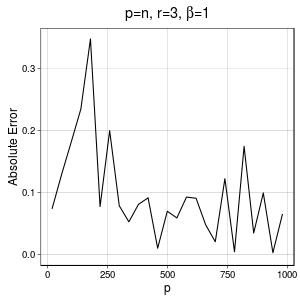
\includegraphics[height=6cm]{code/difference1.jpeg}
%    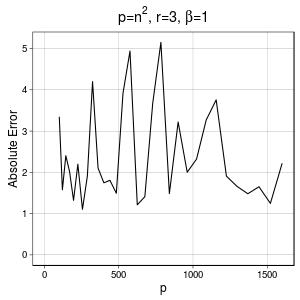
\includegraphics[height=6cm]{code/difference2.jpeg}\\
%    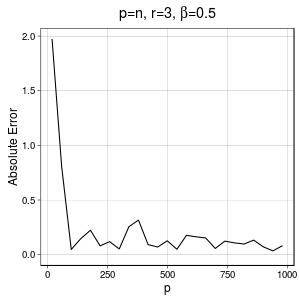
\includegraphics[height=6cm]{code/difference3.jpeg}
%    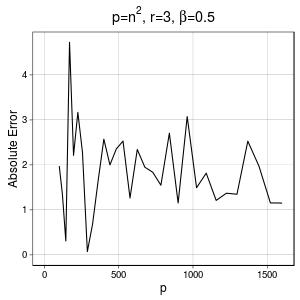
\includegraphics[height=6cm]{code/difference4.jpeg}\\
%    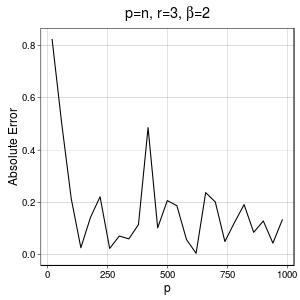
\includegraphics[height=6cm]{code/difference5.jpeg}
%    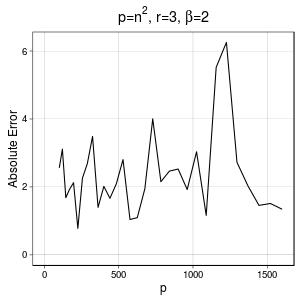
\includegraphics[height=6cm]{code/difference6.jpeg}\\
%    \caption{These are plots of $T_{\textrm{dif}}$ versus $p$. The first column and the second column are the case of $p=n$ and $p=n^2$, separately. The cases of $\beta=1,2,3$ are in the row $1,2,3$ separately. $r$ is set to be $3$ in all cases. }\label{fig:fig1}
%\end{figure}

First, we simulate the level of the new test. We set factor number $r=2$.
Samples are repeatedly generated $1000$ times to calculate empirical level.
For comparison, we also give corresponding `oracle' level which is calculated by `statistics' ${T_1}/(\sigma^2\sqrt{2p\tau^2})$ in equal variance case and ${T_1}/\sqrt{\sigma_n^2}$ in unequal variance case.
The results for equal variance case and unequal variance case are listed in
Table~\ref{biaoge1} and~\ref{biaoge2}, respectively.
From the results, we can find that for small $n$ and $p$, even oracle level is not satisfied.
Level of the new test is a little inflated compared with oracle level.
In all cases, the empirical level tends to be more close to $0.05$ as $n$ increases.

% latex table generated in R 3.3.1 by xtable 1.8-2 package
% Sun Jul 31 01:50:20 2016
\begin{table}[ht]

\caption{Test level simulation. Equal variance case.} 
\label{biaoge1}
    \vspace{3mm}
\centering
\begin{tabular}{rccccccc}
    \toprule
     &  & \multicolumn{2}{c}{$\beta$=0.5} & \multicolumn{2}{c}{$\beta$=1}& \multicolumn{2}{c}{$\beta$=2}   \\
    \cmidrule(r){3-4}
    \cmidrule(r){5-6}
    \cmidrule(r){7-8}
$n$ & $p$ & NEW & ORACLE & NEW & ORACLE & NEW & ORACLE \\ 
\midrule
300 & 200 & 0.075 & 0.062 & 0.079 & 0.062 & 0.074 & 0.070 \\ 
  300 & 400 & 0.074 & 0.065 & 0.061 & 0.044 & 0.046 & 0.040 \\ 
  300 & 600 & 0.058 & 0.041 & 0.070 & 0.052 & 0.071 & 0.055 \\ 
  300 & 800 & 0.066 & 0.047 & 0.071 & 0.052 & 0.062 & 0.048 \\ 
  600 & 200 & 0.061 & 0.055 & 0.052 & 0.051 & 0.058 & 0.056 \\ 
  600 & 400 & 0.051 & 0.048 & 0.051 & 0.042 & 0.059 & 0.051 \\ 
  600 & 600 & 0.061 & 0.058 & 0.056 & 0.054 & 0.051 & 0.047 \\ 
  600 & 800 & 0.053 & 0.046 & 0.060 & 0.050 & 0.056 & 0.048 \\ 
   \bottomrule
\end{tabular}
\end{table}

% latex table generated in R 3.3.3 by xtable 1.8-2 package
% Thu Jun  1 20:35:00 2017
\begin{table}[ht]

\caption{Test level simulation. Unequal variance case.} 
\label{biaoge2}
    \vspace{3mm}
\centering
\begin{tabular}{rccccccc}
  \toprule
    &  & \multicolumn{2}{c}{$\beta$=0.5} & \multicolumn{2}{c}{$\beta$=1}& \multicolumn{2}{c}{$\beta$=2}   \\
    \cmidrule(r){3-4}
    \cmidrule(r){5-6}
    \cmidrule(r){7-8}
$n$ & $p$ & NEW & ORACLE & NEW & ORACLE & NEW & ORACLE \\ 
\midrule
300 & 200 & 0.066 & 0.058 & 0.057 & 0.054 & 0.054 & 0.050 \\ 
  300 & 400 & 0.063 & 0.047 & 0.063 & 0.047 & 0.069 & 0.052 \\ 
  300 & 600 & 0.070 & 0.058 & 0.091 & 0.059 & 0.086 & 0.053 \\ 
  300 & 800 & 0.069 & 0.040 & 0.097 & 0.055 & 0.083 & 0.056 \\ 
  600 & 200 & 0.054 & 0.056 & 0.049 & 0.049 & 0.052 & 0.051 \\ 
  600 & 400 & 0.060 & 0.054 & 0.067 & 0.059 & 0.060 & 0.055 \\ 
  600 & 600 & 0.041 & 0.034 & 0.069 & 0.062 & 0.055 & 0.049 \\ 
  600 & 800 & 0.077 & 0.063 & 0.066 & 0.058 & 0.071 & 0.058 \\ 
   \bottomrule
\end{tabular}

\end{table}




Next, we simulate the empirical power of the new test.
The simulation results of~\cite{Ma2015A} have showed that the level of the~\cite{Chen2010A}'s test can't be guaranteed when covariance is spiked.
To be fair,  critical values are all determined by permutation method.
We set $\Sigma_1=\Sigma_2$, under which permutation method can produce exact test procedures, see~\cite{Lehmann}'s Example 15.2.2.\@
%Note that the statistics of~\cite{Chen2010A},~\cite{Bai1996Efiect} and~\cite{Ma2015A} all produce the same permutation test.
%Indeed, they are all equivalent to the permutation test based on $\|\bar{X}_1-\bar{X}_2\|^2$.
We permutate the sample $100$ times to determine the critical value. We repeat the test procedure $500$ times to obtain empirical power.
We plot the empirical power versus signal-to-noise ratio $\textrm{SNR}=\|\mu_1-\mu_2\|^2/(\sigma^2\sqrt{2\tau^2 p})$.
The results are illustrated in figure~\ref{fig:fig1} and~\ref{fig:fig2}, where `NEW', `CQ' and `S' represent the new test,~\cite{Chen2010A}'s test and \cite{Srivastava2008A}'s test.
From the results, we can find that when $\Sigma$ is spiked, the new test outperforms $T_{CQ}$ substantially; when $\Sigma$ is not spiked, all three tests have similar performance.
\begin{figure}
    \centering 
    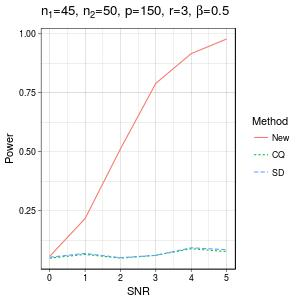
\includegraphics[height=6cm]{code/fig1.jpeg}
    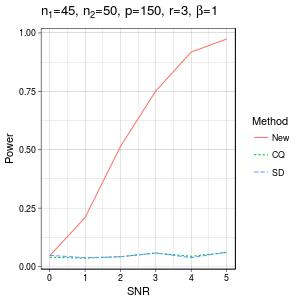
\includegraphics[height=6cm]{code/fig2.jpeg}
    \\
    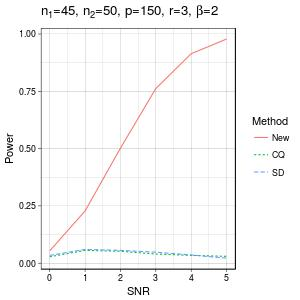
\includegraphics[height=6cm]{code/fig3.jpeg}
    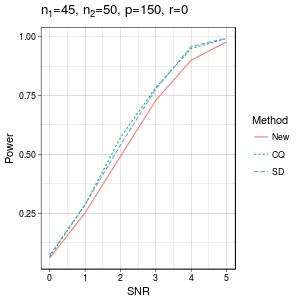
\includegraphics[height=6cm]{code/fig4.jpeg}
    \caption{Empirical power simulation.}\label{fig:fig1}
\end{figure}

\begin{figure}
    \centering 
    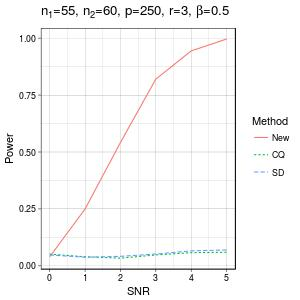
\includegraphics[height=6cm]{code/fig5.jpeg}
    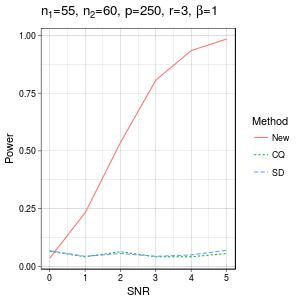
\includegraphics[height=6cm]{code/fig6.jpeg}
    \\
    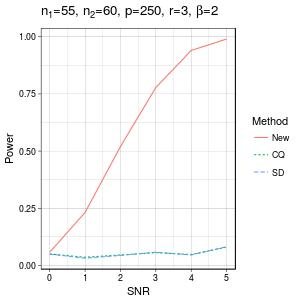
\includegraphics[height=6cm]{code/fig7.jpeg}
    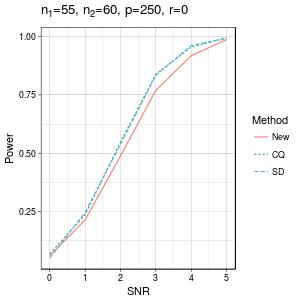
\includegraphics[height=6cm]{code/fig8.jpeg}
    \caption{Empirical power simulation.}\label{fig:fig2}
\end{figure}
%Permutation method is computation expensive. So when $p$ and $n$ are large, we simulate empirical power by asymptotic distribution. The results are illustrated in figure~\eqref{fig:fig3}.

%\begin{figure}\label{fig:fig3}
    %\centering 
    %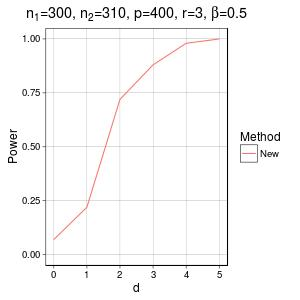
\includegraphics[height=6cm]{code/newfig1.jpeg}
    %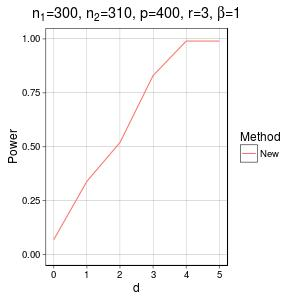
\includegraphics[height=6cm]{code/newfig2.jpeg}
    %\\
    %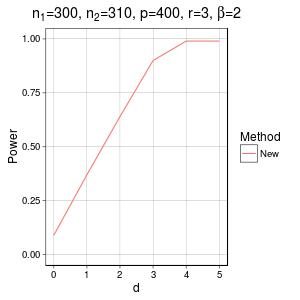
\includegraphics[height=6cm]{code/newfig3.jpeg}
    %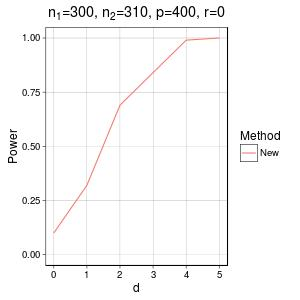
\includegraphics[height=6cm]{code/newfig4.jpeg}
    %\\
    %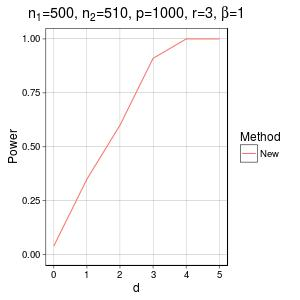
\includegraphics[height=6cm]{code/newfig5.jpeg}
    %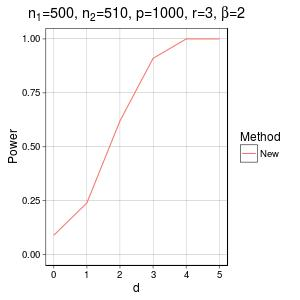
\includegraphics[height=6cm]{code/newfig6.jpeg}
    %\caption{Empirical Power (critical values are computed by asymptotic distribution)}\label{fig:fig3}
%\end{figure}

\subsection{Real data analysis}
In this section, we study the practical problem considered in~\cite{Ma2015A}.
The task is to test whether Monday stock returns are equal to those of other trading days on average.
Define an observation be the log return of stocks in a day.
Hence $p$ is the total number of stocks.
Let sample $1$ and sample $2$ be the observations on Monday and the other trading days, respectively.
Then we would like to test $H_0\, :\mu_1=\mu_2$ v.s. $H_1\,:\mu_1\neq \mu_2$.
We collected the data of $p=710$
 stocks of China
from 01/04/2013 to 12/31/2014. There are total $n_1=95$ Monday and $n_2=388$ other trading days. 

We assume $\Sigma_1=\Sigma_2$.
The first eigenvaule of $S$ is $0.14$, which is significantly larger than the others.
In fact, the second eigenvalue is $0.02$.
Hence there's clearly a spiked eigenvalue.
We set $r=1$ and perform our new test.
The $p$ value is $0.149$, which is obtained by $1000$ permutations.
Hence, the null hypothesis can not be rejected for $\alpha=0.05$.
We draw the same conclusion as~\cite{Ma2015A}.

\section{Conclusion remark}



This paper is concerned with the problem of testing the equality of means in the setting of high dimension and spiked covariance. We drop big variance terms from $T_{CQ}$ and obtain a new test statistic. The asymptotic normality of the new statistic is proved and the asymptotic power is given. %The new test outperforms $T_{CQ}$ substantially if the variance is spiked.

%We also generalize the test to unequal variance case.

In another paper,~\cite{Zhao2016A} proved that their test statistic can be written in the form of projection. Their simulation results showed that their test performs well under strong correlations.
Our work partially explains why their test performs well although the projections are slightly different. 

 Spiked covariance is an important correlation pattern and has been widely studied in terms of PCA\@.
 In PCA, authors focus on the principal subspace.
 However, in some circumstances, as our work have shown, the complement of principal subspace is more useful. 

In our paper, we have assumed $r$ is known. If $r$ is an unknown positive number, a consistent estimator of $r$ is
\begin{equation}\label{estimateR}
    \hat{r}=\textrm{argmax}_{l\leq R}\frac{\lambda_l(S)}{\lambda_{l+1}(S)},
\end{equation}
where $R$ is a hyperparameter.
    See~\cite{Ahn2009Eigenvalue} for detail.


Our theoretical results rely on the assumption $\sqrt{p}/n\to 0$. In the situation of small sample or very large $p$, the critical value of the new test can be determined by permutation method. Our simulation shows that the new test still performs well. It remains a theoretical interest to study the asymptotic behavior of permutation based test in these situations.



\section*{Appendix}

%\begin{lemma}\label{lemma1}
%    let $X$ be a $p$-dimensional random vector with distribution $N(0,\Sigma)$. Denote the spectral decomposition of $\Sigma$ by $\Sigma =\sum_{i=1}^p \lambda_i p_i p_i^T$ with $\lambda_1\geq \cdots \geq \lambda_p$. Then $X^T p_i p_i^T X$ is stochastically larger than $X^T p_j p_{j}^T X$ for $i<j$.
%\end{lemma}
%\begin{proof}[\textbf{Proof}]
%    The lemma is established immediately once we note that $X^T p_i p_i^T X/\sqrt{\lambda_i}$ is distributed as $\chi^2$ distribution with freedom $1$.
%\end{proof}

\begin{lemma}[Weyl's inequality]
Let $H$ and $P$ be two symmetric $n\times n$ matrices and $M=H+P$. If $r+s-1 \leq  i\leq j+k-n$, we have
\begin{equation*}
\lambda_j(H)+\lambda_k(P)\leq \lambda_i(M) \leq \lambda_r(H)+\lambda_s(P).
\end{equation*}
    See, for example,~\cite{Horn1985Matrix} Theorem $4.3.1$.
\end{lemma}
%\begin{corollary}\label{WeylCor}
    %Let $H$ and $P$ be two symmetric matrices and $M=H+P$. If $\mathrm{rank}(P)< k\leq n$, then
    %\begin{equation*}
        %\lambda_k(M)\leq \lambda_1(H).
    %\end{equation*}
%\end{corollary}


\begin{lemma}[Convergence rate of principal space estimation]\label{conRateLemma}
    Under the Assumption~\ref{theModel}, we have
\begin{equation*}
E\|\hat{V}\hat{V}^T-VV^T\|^2_F =O(\frac{p}{p^{\beta}n}).
\end{equation*}
\end{lemma}


\begin{proof}[\textbf{Proof}]
    Theorem 5 of~\cite{Cai2012Sparse} asserts that sample principal subspace $\hat{V}\hat{V}^T$ is a minimax rate optimal estimator of $VV^T$, namely, it reaches the minimax convergence rate
    \begin{equation}\label{xiaopianpian}
         E\|\hat{V}\hat{V}^T-VV^T\|^2_F\asymp r\wedge (p-r)\wedge \frac{r(p-r)}{(n_1+n_2-2)p^\beta}
    \end{equation}
    as long as the right hand side tends to $0$. 
    It's obvious that the right hand side of~\eqref{xiaopianpian} is of order ${p^{1-\beta}}/{n}$.
\end{proof}
\begin{lemma}[Bai-Yin's law]\label{baiyin}
    Suppose $B_n=\frac{1}{q} Z Z^T$ where $Z$ is $p\times q$ random matrix composed of i.i.d.\ random variables with zero mean, unit variance and finite fourth moment.
    As $q\to \infty$ and $\frac{p}{q}\to c\in [0,\infty)$, the largest and smallest non-zero eigenvalues of $B_n$ converge almost surely to ${(1+\sqrt{c})}^2$ and $(1-\sqrt{c})^2$, respectively.
\end{lemma}
\begin{remark}
    Lemma~\ref{baiyin} is known as the Bai-Yin's law (\cite{bai1993limit}). As in Remark $1$ of~\cite{bai1993limit}, the smallest non-zero eigenvalue is the $p-q+1$ smallest eigenvalue of $B$ for $c>1$.
\end{remark}

\begin{corollary}\label{maxEigen}
    Suppose that $W_n$ is a $p \times p$ matrix distributed as $\mathrm{Wishart}_p(n,I_{p})$ where $\operatorname{Wishart}_p(m,\Psi)$ is the $p$ dimensional Wishart distribution with parameter $\Psi$ and $m$ degrees of freedom. Then as $n,p\to \infty$,
    $$
        \lambda_1(W_n)=O_P(\max(n,p)).
    $$
\end{corollary}
\begin{proof}[\textbf{Proof}]
    Since $[0,+\infty]$ is compact, for every subsequance $\{n_{k}\}$ of $\{n\}$, there is a further subsequance $\{n_{k_l}\}$ along which $p/n\to c\in [0,+\infty]$.

    If $c\in [0,+\infty)$, by Lemma~\ref{baiyin}, we have that
    $$
    \frac{\lambda_1(W_{n_{k_l}})}{n_{k_l}}\xrightarrow{P}{(1+c)}^2.
    $$
    Hence the conclusion holds along this subsequance.
    If $c=+\infty$, suppose $W_n=Z_n Z_n^T$ where $Z_n$ is a $p\times n$ matrix with all elements independently distributed as $N(0,1)$. Then
    $$
    \frac{\lambda_1(W_{n_{k_l}})}{p}=\frac{\lambda_1(Z_{n_{k_l}}^T Z_{n_{k_l}})}{p}\xrightarrow{P} 1
    $$
    by Lemma~\ref{baiyin}, which proves the conclusion along the subsequance. Now the conclusion holds by a standard subsequance argument.
\end{proof}


\begin{proof}[\textbf{Proof of Proposition~\ref{quadraticFormCLT}}]
    Let $\lambda_1(A_n)\geq\cdots\geq \lambda_{k_n}(A_n)$ be the eigenvalues of $A_n$, then 
    \begin{equation}
        \frac{Y_n^T A_n Y_n-\mathrm{E} Y_n^T A_n Y_n}{{[\mathrm{Var}(Y_n^T A_n Y_n)]}^{1/2}}=\sum_{i=1}^{k_n}\frac{\lambda_i(A_n)}{{\big[2\mathrm{tr}(A_n^2)\big]}^{1/2}}(Z_{ni}^2-1),
    \end{equation}
    where $Z_{ni}$'s ($i=1,\ldots,k_n$) are independent standard normal random variables.

    If~\ref{quadraticEigen} holds, then
    \begin{equation*}
        \begin{aligned}
            &\sum_{i=1}^{k_n}\mathrm{E}\Big[\frac{\lambda_i^2(A_n)}{2\mathrm{tr}(A_n^2)}{(Z_{ni}^2-1)}^2\Big\{\frac{\lambda_i^2(A_n)}{2\mathrm{tr}(A_n^2)}{(Z_{ni}^2-1)}^2\geq \epsilon\Big\}\Big]\\
            \leq&\sum_{i=1}^{k_n}
            \frac{\lambda_i^2(A_n)}{2\mathrm{tr}(A_n^2)}
            \mathrm{E}\Big[{(Z_{n1}^2-1)}^2\Big\{\frac{\lambda_{\max}(A_n^2)}{2\mathrm{tr}(A_n^2)}{(Z_{n1}^2-1)}^2\geq \epsilon\Big\}\Big]\\
            =&
            \frac{1}{2}\mathrm{E}\Big[{(Z_{n1}^2-1)}^2\Big\{\frac{\lambda_{\max}(A_n^2)}{2\mathrm{tr}(A_n^2)}{(Z_{n1}^2-1)}^2\geq \epsilon\Big\}\Big]\to 0.
        \end{aligned}
    \end{equation*}
    Hence~\ref{quadratic} follows by Lindeberg's central limit theorem.

    Conversely, if~\ref{quadratic} holds, we will prove that there is a subsequence of $\{n\}$ along which~\ref{quadraticEigen} holds. Then~\ref{quadraticEigen} will hold by a standard contradiction argument. 

    Denote $c_{ni}=\lambda_i(A_n)/{\big[2\mathrm{tr}(A_n^2)\big]}^{1/2}$ ($i=1,\ldots,k_n$), we have $c_{ni}\in[-\sqrt{2}/2,\sqrt{2}/2]$.
    Since~\ref{quadratic} holds, the characteristic function of
        $
        \sum_{i=1}^{k_n}c_{ni}(Z_{ni}^2-1)
    $
    converges to $\exp(-t^2/2)$ for every $t$. For $t\in (-1,1)$, we have
    \begin{equation*}
        \begin{aligned}
            &\log \mathrm{E}\exp{\big(it \sum_{j=1}^{k_n}c_{nj}(Z_{nj}^2-1)\big)}
            =
            -i(\sum_{j=1}^{k_n}c_{nj})t-
            \frac{1}{2}\sum_{j=1}^{k_n}\log(1-i2c_{nj}t)\\
            =&
            -i(\sum_{j=1}^{k_n}c_{nj})t+
            \frac{1}{2}\sum_{j=1}^{k_n}\sum_{l=1}^{+\infty}\frac{1}{l}{(i2c_{nj}t)}^l
            =
            -i(\sum_{j=1}^{k_n}c_{nj})t+
            \frac{1}{2}\sum_{l=1}^{+\infty}\Big[\sum_{j=1}^{k_n}{(c_{nj})}^l\Big]\frac{1}{l}{(i2t)}^l\\
            =&-\frac{1}{2}t^2+
            \frac{1}{2}\sum_{l=3}^{+\infty}\Big[\sum_{j=1}^{k_n}{(c_{nj})}^l\Big]\frac{1}{l}{(i2t)}^l.
        \end{aligned}
    \end{equation*}
    Denote $b_{nl}=\sum_{j=1}^{k_n}{(c_{nj})}^l$, $n=1,2,\cdots$ and $l=3,4,\cdots$. For $l\geq 3$, $\big|\sum_{j=1}^{k_n}{(c_{nj})}^l\big|\leq \big|\sum_{j=1}^{k_n}{(c_{nj})}^2\big|=1/2$.
    By Helly's selection theorem, there's a subsequence of $\{n\}$ along which $\lim_{n\to \infty}b_{nl}=b_l$ exists for every $l$.
    Apply dominated convergence theorem to this subsequence we have
            $\log \mathrm{E}\exp{\big(it \sum_{j=1}^{k_n}c_{nj}(Z_{nj}^2-1)\big)}\to
            -\frac{1}{2}t^2+
            \frac{1}{2}\sum_{l=3}^{+\infty}b_l\frac{1}{l}{(i2t)}^l$ for $t\in(-1/2,1/2)$.
            By the property of power series, we have $b_l=0$ for $l\geq 3$. Then~\ref{quadraticEigen} follows by noting that $b_{n4}\geq \max_j{(c_{nj})}^4$.
\end{proof}




The rest of the Appendix is devoted to the proof of propositions and theorems in the paper.

\begin{proof}[\textbf{Proof of Theorem~\ref{Chenstheory}}]
    Note that $(n_k-1)S_k\sim \text{Wishart}_p(n_k-1,\Sigma)$, $k=1,2$, we have %$(n_1-1)\mytr S_1\sim \sum_{i=1}^{p} \lambda_i (\Sigma) W_i$ where $W_i\sim \chi^2_{n_1-1} $.
    %Note that $\lambda_{r+1}(\Sigma)=\cdots=\lambda_p(\Sigma)=\sigma^2$, by central limit theorem, we have
    %$$
    %\begin{aligned}
        %&\sum_{i=1}^{p} \lambda_i (\Sigma) W_i=
    %\sum_{i=1}^{r} \lambda_i (\Sigma) W_i+
    %\sum_{i=r+1}^{p} \sigma^2 W_i\\
        %\sim&
    %\sum_{i=1}^{r} \lambda_i (\Sigma) W_i+
        %(p-r)(n_1-1)\sigma^2+
        %\sqrt{(n_1-1)(p-r)}\sigma^2\epsilon+o_P(\sqrt{np}),
    %\end{aligned}
    %$$
    %where $\epsilon\sim N(0,1)$. By law of large numbers, we have $W_i/(n_i-1)\xrightarrow{P}1$. Hence
%$$
%\begin{aligned} 
    %\frac{1}{\tau p^{\beta} n_1}\mytr S_1
    %&\sim
    %\frac{1}{\tau n_1}\sum_{i=1}^{r} \frac{\lambda_i +\sigma^2}{p^{\beta}} \frac{W_i}{n_i-1}+
        %\frac{p-r}{\tau p^{\beta}n_1}\sigma^2+
        %\frac{1}{\tau p^\beta n_1}\sqrt{\frac{p-r}{n_1-1}}\sigma^2\epsilon+o_P(n^{-1/2}p^{1/2-\beta})\\
        %&=
    %\frac{1}{\tau n_1}\sum_{i=1}^{r} l_i+
        %\frac{p-r}{\tau p^{\beta}n_1}\sigma^2+
        %\frac{1}{\tau p^\beta n_1}\sqrt{\frac{p-r}{n_1-1}}\sigma^2\epsilon+o_P(1)\\
%\end{aligned}
%$$
%
    %Hence
    $$
 \myE\Big(\frac{1}{n_1}\mytr S_1+\frac{1}{n_2}\mytr S_2\Big)=\tau \mytr\Sigma,
    $$
    and
    $$
    \begin{aligned}
        &\myVar\Big(\frac{1}{n_1}\mytr S_1+\frac{1}{n_2}\mytr S_2\Big)=
        \Big(\frac{2}{n_1^2(n_1-1)}+\frac{2}{n_2^2(n_2-1)}\Big)\mytr \Sigma^2\\
        =&
    O\Big(\frac{1}{n^3}(p^{2\beta}+p)\Big)=O\Big(\frac{p^{2\beta}}{n^3}\Big).
    \end{aligned}
    $$
    It follows that
    $$
    \begin{aligned}
        &\frac{1}{n_1}\mytr S_1+\frac{1}{n_2}\mytr S_2=
    \tau \mytr \Sigma+O_P\Big(\frac{1}{n\sqrt{n}}p^{\beta}\Big)\\
        =&\tau \sum_{i=1}^r (\lambda_i+\sigma^2)+\tau(p-r)\sigma^2+O_P\Big(\frac{1}{n\sqrt{n}}p^{\beta}\Big)\\
        =&\tau p^{\beta} \sum_{i=1}^r l_i+\tau(p-r)\sigma^2+o_P\Big(\frac{1}{n}p^{\beta}\Big).
    \end{aligned}
    $$
Thus,
        \begin{equation}\label{eq:kkk1}
        \frac{1}{\tau p^\beta}\big(\frac{1}{n_1}\mytr S_1+\frac{1}{n_2}\mytr S_2\big)
        =\sum_{i=1}^r l_i+p^{1-\beta}\sigma^2+o_P(1).
        \end{equation}

    Next we deal with $\|\bar{X}_1-\bar{X}_2\|^2$.
    Note that we have
    $$
    \|\bar{X}_1-\bar{X}_2\|^2=
    \|V^T(\bar{X}_1-\bar{X}_2)\|^2+
    \|\tilde{V}^T(\bar{X}_1-\bar{X}_2)\|^2.
    $$
    These two terms are independent.
    For the first term, note that $V^T(\bar{X}_1-\bar{X}_2)\sim N_r\big(V^T (\mu_1-\mu_2),\tau (\Lambda+\sigma^2 I_r)\big)$, we have
    $$
    \begin{aligned}
        \|V^T(\bar{X}_1-\bar{X}_2)\|^2&\sim
        \sum_{i=1}^r \Big(\sqrt{\tau (\lambda_i+\sigma^2)}Z_i+\big(V^T (\mu_1-\mu_2)\big)_i \Big)^2\\
        &=\tau p^{\beta}
        \sum_{i=1}^r
        \Big( \sqrt{p^{-\beta}(\lambda_i+\sigma^2)}Z_i+\frac{1}{\sqrt{\tau p^{\beta}}}\big(V^T (\mu_1-\mu_2)\big)_i \Big)^2.
    \end{aligned}
    $$
    By the assumptions of the theorem,  we have that
    \begin{equation}\label{eq:kkk2}
    \begin{aligned}
        \frac{1}{\tau p^{\beta}}\|V^T(\bar{X}_1-\bar{X}_2)\|^2
        \xrightarrow{\mathcal{L}}
        \sum_{i=1}^r (l_i Z_i+\zeta_i)^2.
    \end{aligned}
    \end{equation}

    As for $\|\tilde{V}^T(\bar{X}_1-\bar{X}_2)\|^2$, we have that
    \begin{equation}\label{prop1eq1}
        \begin{aligned}
            &\|\tilde{V}^T(\bar{X}_1-\bar{X}_2)\|^2
            =\big\|\tilde{V}^T(\mu_1-\mu_2)+\tilde{V}^T\big((\bar{X}_1-\mu_1)-(\bar{X}_2-\mu_2)\big)\big\|^2\\
            =&\|\tilde{V}^T(\mu_1-\mu_2)\|^2+
            \big\|\tilde{V}^T\big((\bar{X}_1-\mu_1)-(\bar{X}_2-\mu_2)\big)\big\|^2+
            2{(\mu_1-\mu_2)}^T\tilde{V}\tilde{V}^T\big((\bar{X}_1-\mu_1)-(\bar{X}_2-\mu_2)\big).
        \end{aligned}
    \end{equation}
Since $\tilde{V}^T (\bar{X}_1-\bar{X}_2)\sim N_{p-r}(\tilde{V}^T (\mu_1-\mu_2),  \sigma^2 \tau I_{p-r})$, by central limit theorem, we have
    $$
\frac{
    \big\|\tilde{V}^T\big((\bar{X}_1-\mu_1)-(\bar{X}_2-\mu_2)\big)\big\|^2-\sigma^2 \tau (p-r)}{\sigma^2 \tau\sqrt{2(p-r)}}\xrightarrow{\mathcal{L}} N(0,1).
    $$
    For the intersection term, we have
    \begin{equation*}
        \begin{aligned}
            &2{(\mu_1-\mu_2)}^T\tilde{V}\tilde{V}^T\big((\bar{X}_1-\mu_1)-(\bar{X}_2-\mu_2)\big)
            \sim N(0,4\sigma^2 \tau \|\tilde{V}^T(\mu_1-\mu_2)\|^2)\\
            =& O_P(\sqrt{\tau}\|\tilde{V}^T(\mu_1-\mu_2)\| )=o_P(\tau p^{\beta}).
        \end{aligned}
    \end{equation*}
    It follows that
    \begin{equation}\label{eq:kkk3}
\frac{1}{\tau p^\beta}
    \big(\big\|\tilde{V}^T(\bar{X}_1-\bar{X}_2)\big\|^2-\sigma^2 \tau (p-r)-\big\|\tilde{V}^T(\mu_1-\mu_2)\big\|^2\big)
    \xrightarrow{\mathcal{L}} 
    \sqrt{2}\sigma^2 \delta_{\{\frac{1}{2}\}}(\beta)\epsilon.
    \end{equation}


    Combining~\eqref{eq:kkk1}~\eqref{eq:kkk2} and~\eqref{eq:kkk3} leads to
    $$
    \begin{aligned}
        &\frac{1}{\tau p^{\beta}} T_{CQ}
        =\frac{1}{\tau p^{\beta}}\big(\|\bar{X}_1-\bar{X}_2\|^2-\frac{1}{n_1}\mytr S_1-\frac{1}{n_2}\mytr S_2\big)\\
        =&
        \frac{1}{\tau p^{\beta}}{\|V^T(\bar{X}_1-\bar{X}_2)\|^2}+
        \frac{1}{\tau p^{\beta}} \big({\|\tilde{V}^T(\bar{X}_1-\bar{X}_2)\|^2-\sigma^2 \tau(p-r)-\|\tilde{V}^T(\mu_1-\mu_2)\|^2}\big)\\
        &-\frac{1}{\tau p^{\beta}}\Big(\frac{1}{n_1}\mytr S_1+\frac{1}{n_2}\mytr S_2\Big)+\frac{\sigma^2 (p-r)}{p^\beta}+\frac{1}{\tau p^\beta}\|\tilde{V}^T(\mu_1-\mu_2)\|^2\\
        =&
        \sum_{i=1}^r (l_i Z_i+\zeta_i)^2+
   \sqrt{2} \sigma^2 \delta_{\{\frac{1}{2}\}}(\beta)\epsilon
        -
        (\sum_{i=1}^r l_i+p^{1-\beta}\sigma^2)
        +\frac{\sigma^2 (p-r)}{p^\beta}+\zeta^*+o_P(1)\\
        \xrightarrow{\mathcal{L}}&
        \sum_{i=1}^r (l_i Z_i+\zeta_i)^2+
\zeta^*+
    \sqrt{2}\sigma^2 \delta_{\{\frac{1}{2}\}}(\beta)\epsilon
        -
        \sum_{i=1}^r l_i.
    \end{aligned}
    $$
    This completes the proof.

    %Note that we have $\|\bar{X}_1-\bar{X}_2\|^2\sim \tau(\sum_{i=1}^r \lambda_i(\Sigma)Z_i+\sigma^2 W)$, where $Z_i\overset{i.i.d.}{\sim}\chi^2_1$ and $W\sim \chi^2_{p-r}$ is independent of $Z_i$'s. Then
    %$$
    %\frac{1}{\tau p^{\beta}}\|\bar{X}_1-\bar{X}_2\|^2
    %\sim\sum_{i=1}^r\frac{\lambda_i+\sigma^2}{p^{\beta}}Z_i
    %+\frac{\sigma^2}{p^{\beta}}W.
    %$$
    %It's easy to see that 
    %$$\sum_{i=1}^r\frac{\lambda_i+\sigma^2}{p^{\beta}}Z_i\xrightarrow{\mathcal{L}}\sum_{i=1}^r l_i Z_i.$$
    %By central limit theorem, we have
    %$$
    %\frac{1}{\sqrt{2(p-r)}}\big( W-(p-r)\big)\xrightarrow{\mathcal{L}}N(0,1).
    %$$
%
    %If $\beta=1/2$, by Slutsky's theorem we have
    %$$
    %\frac{1}{\tau p^{\beta}}\|\bar{X}_1-\bar{X}_2\|^2-\frac{\sigma^2(p-r)}{p^\beta}\xrightarrow{\mathcal{L}}
    %\sum_{i=1}^r l_i Z_i+\sqrt{2}\sigma^2 \epsilon.
    %$$
    %where $\epsilon\sim N(0,1)$

\end{proof}


\begin{proof}[\textbf{Proof of Proposition~\ref{oracleTheorem}}]
Note that
    \begin{equation}
        \begin{aligned}
            &\|\tilde{V}^T(\bar{X}_1-\bar{X}_2)\|^2
            =\big\|\tilde{V}^T(\mu_1-\mu_2)+\tilde{V}^T\big((\bar{X}_1-\mu_1)-(\bar{X}_2-\mu_2)\big)\big\|^2\\
            =&\|\tilde{V}^T(\mu_1-\mu_2)\|^2+
            \big\|\tilde{V}^T\big((\bar{X}_1-\mu_1)-(\bar{X}_2-\mu_2)\big)\big\|^2+
            2{(\mu_1-\mu_2)}^T\tilde{V}\tilde{V}^T\big((\bar{X}_1-\mu_1)-(\bar{X}_2-\mu_2)\big)\\
            =&\|\tilde{V}^T(\mu_1-\mu_2)\|^2+
            \big\|\tilde{V}^T\big((\bar{X}_1-\mu_1)-(\bar{X}_2-\mu_2)\big)\big\|^2+
            o_P(\frac{\sqrt{p}}{n}).
        \end{aligned}
    \end{equation}
    The last equality holds since
    \begin{equation*}
        \begin{aligned}
            &2{(\mu_1-\mu_2)}^T\tilde{V}\tilde{V}^T\big((\bar{X}_1-\mu_1)-(\bar{X}_2-\mu_2)\big)\sim N(0,4\sigma^2 \tau \|\tilde{V}^T(\mu_1-\mu_2)\|^2)\\
            =& O_P(\sqrt{\tau}\|\tilde{V}^T(\mu_1-\mu_2)\| )=o_P(\frac{\sqrt{p}}{n}).
        \end{aligned}
    \end{equation*}

    %Let $Y_{k,i}=\tilde{V}^T (X_{k,i}-\mu_k)$, $i=1,\ldots,n_k$, $k=1,2$.
    %Then $Y_{k,i}\sim N(\tilde{V}^T\mu_k,\sigma^2 I_{p-r})$.
    %Let $\bar{Y}_1$ and $\bar{Y}_2$ be the sample means of $\{Y_{1,i}\}_{i=1}^{n_1}$ and $\{Y_{2,i}\}_{i=1}^{n_2}$ respectively. 
    %Then
    %\begin{equation}\label{prop1eq1}
        %\begin{aligned}
            %&\|\tilde{V}^T(\bar{X}_1-\bar{X}_2)\|^2
            %=\|\tilde{V}^T(\mu_1-\mu_2)+(\bar{Y}_1-\bar{Y}_2)\|^2\\
            %=&\|\tilde{V}^T(\mu_1-\mu_2)\|^2+\|\bar{Y}_1-\bar{Y}_2\|^2+
            %2{(\mu_1-\mu_2)}^T\tilde{V}(\bar{Y}_1-\bar{Y}_2)\\
            %=&\|\tilde{V}^T(\mu_1-\mu_2)\|^2+\|\bar{Y}_1-\bar{Y}_2\|^2+
            %o_P(\frac{\sqrt{p}}{n}).
        %\end{aligned}
    %\end{equation}
    %The last equality holds since
    %\begin{equation*}
        %\begin{aligned}
            %&2{(\mu_1-\mu_2)}^T\tilde{V}(\bar{Y}_1-\bar{Y}_2)\sim N(0,4\sigma^2 \tau \|\tilde{V}^T(\mu_1-\mu_2)\|^2)\\
            %=& O_P(\sqrt{\tau}\|\tilde{V}^T(\mu_1-\mu_2)\| )=o_P(\frac{\sqrt{p}}{n}).
        %\end{aligned}
    %\end{equation*}
    For $k=1,2$, we have
    %${n_k^{-1}} \tilde{V}^T S_k \tilde{V}\sim
    %\frac{\sigma^2}{n_k(n_k-1)}\operatorname{Wishart}_{p-r}(n_k-1,I_{p-r})
    %$, $k=1,2$.
    %Then 
    \begin{equation*}
        \begin{aligned}
            &\frac{1}{n_k} \mathrm{tr}(\tilde{V}^T S_k \tilde{V})\sim \frac{\sigma^2}{n_k(n_k-1)}\chi^2_{(p-r)(n_k-1)}
            =
            \sigma^2\frac{p-r}{n_k}\Big(1+O_P\big(\frac{1}{\sqrt{(p-r)(n_k-1)}}\big)\Big),
        \end{aligned}
    \end{equation*}
    where the last equality comes from central limit theorem. It follows that
    \begin{equation}\label{prop1eq2}
        \begin{aligned}
            &\frac{1}{n_1} \mathrm{tr}(\tilde{V}^T S_1 \tilde{V})+
            \frac{1}{n_2} \mathrm{tr}(\tilde{V}^T S_2 \tilde{V})=\sigma^2 \tau (p-r)+o_P(\frac{\sqrt{p}}{n}).
        \end{aligned}
    \end{equation}

    Equation~\eqref{prop1eq1} and~\eqref{prop1eq2} imply that
    \begin{equation}
        \begin{aligned}
            \frac{T_1-\|\tilde{V}^T(\mu_1-\mu_2)\|^2}{\sigma^2\sqrt{2\tau^2 p}}
            =
            \frac{\|\bar{Y}_1-\bar{Y}_2\|^2-
                \sigma^2 \tau (p-r)}{\sigma^2\sqrt{2\tau^2 p}}
                +o_P(1).
        \end{aligned}
    \end{equation}
    Since
$\|\tilde{V}^T(\bar{Z}_1-\bar{Z}_2)\|^2\sim \sigma^2\tau\chi^2_{p-r}$,
the proposition follows by central limit theorem.
\end{proof}



\begin{proof}[\textbf{Proof of Proposition~\ref{varianceEstimation}}]
    Note that $(n-2)S\sim \mathrm{Wishart}_p (n-2,\Sigma)$.
    Denote by $\Sigma=UEU^T$ the spectral decomposition of $\Sigma$, where $U=(V,\tilde{V})$ is an orthogonal matrix and $E=\mathrm{diag}(\lambda_1+\sigma^2,\ldots,\lambda_r+\sigma^2,\sigma^2,\ldots,\sigma^2)$.
    Let $Z$ be a $p\times (n-2)$ random matrix with all elements i.i.d.\ distributed as $N(0,1)$, then
    $$
        S\sim \frac{1}{n-2} U E^{1/2} Z Z^T E^{1/2} U^T.
    $$
    Thus,
    \begin{equation*}
        \begin{aligned}
            \hat{\sigma}^2\sim
            \frac{1}{(p-r)(n-2)}\sum_{i=r+1}^p \lambda_i (U E^{1/2} Z Z^T E^{1/2} U^T)
            =
            \frac{1}{(p-r)(n-2)}\sum_{i=r+1}^{n-2} \lambda_i ( Z^T E Z).
        \end{aligned}
    \end{equation*}
    Denote $Z={(Z_{(1)}^T,Z_{(2)}^T)}^T$, where $Z_{(1)}$ and $Z_{(2)}$ are the first $r$ rows and last $p-r$ rows of $Z$. We have
    $$
    Z^T E Z =Z_{(1)}^T (\Lambda +\sigma^2 I_r) Z_{(1)}+\sigma^2 Z_{(2)}^T Z_{(2)}.
    $$
 The first term is of rank $r$. By Weyl's inequality, we have
    $$
    \sigma^2\lambda_i(Z_{(2)}^T Z_{(2)}) \leq \lambda_i(Z^T E Z)\leq
    \sigma^2\lambda_{i-r}(Z_{(2)}^T Z_{(2)}),
    \quad
    \textrm{$i=r+1,\ldots, n-2$}.
    $$
    Thus,
    $$
    \sigma^2\sum_{i=r+1}^{n-2}\lambda_i(Z_{(2)}^T Z_{(2)}) \leq \sum_{i=r+1}^{n-2}\lambda_i(Z^T E Z)\leq
    \sigma^2\sum_{i=1}^{n-r-2}\lambda_{i}(Z_{(2)}^T Z_{(2)}).
    $$
     It follows that
     \begin{equation*}
         \begin{aligned}
             &\Big|\frac{1}{(p-r)(n-2)}\sum_{i=r+1}^{n-2}\lambda_i(Z^T E Z)-
    \frac{1}{(p-r)(n-2)} \sigma^2\sum_{i=1}^{n-2}\lambda_{i}(Z_{(2)}^T Z_{(2)})\Big|
             \\
             \leq & r\sigma^2\frac{1}{(p-r)(n-2)} \lambda_1 (Z_{(2)}^T Z_{(2)}).
         \end{aligned}
     \end{equation*}
    By Corollary~\ref{maxEigen}, $\lambda_1 (Z_{(2)}^T Z_{(2)})=O_P(\max(n,p))$. 
    Thus,
     \begin{equation*}
         \begin{aligned}
             &\frac{1}{(p-r)(n-2)}\sum_{i=r+1}^{n-2}\lambda_i(Z^T E Z)\\
             =&
    \frac{1}{(p-r)(n-2)} \sigma^2\sum_{i=1}^{n-2}\lambda_{i}(Z_{(2)}^T Z_{(2)})
             +O_P(\frac{\max(n,p)}{np})\\
             =&
             \frac{1}{(p-r)(n-2)} \sigma^2\mathrm{tr}(Z_{(2)}^T Z_{(2)})
             +O_P(\frac{\max(n,p)}{np})\\
             =&
             \sigma^2
                +O_P(\frac{1}{\sqrt{np}})
             +O_P(\frac{\max(n,p)}{np}).\\
         \end{aligned}
     \end{equation*}
     The last equality comes from central limit theorem.
The theorem follows by noting that
$$
    O_{P}(\frac{1}{\sqrt{np}})=O_P(\frac{\sqrt{np}}{np})= O_P(\frac{\max (n,p)}{np}).
$$
\end{proof}



% proof of space estimation theorem
\begin{proof}[\textbf{Proof of Theorem~\ref{myPanpan}}]

    Note that $\mathrm{tr}(\hat{\tilde{V}}^T S_k\hat{\tilde{V}})=\sum_{i=r+1}^p \lambda_i(S_k)$, $k=1,2$.
    Similar to Proposition~\ref{varianceEstimation}, we have $\mathrm{tr}(\hat{\tilde{V}}^T S_k\hat{\tilde{V}})=(p-r)\sigma^2+O_P({\max(n,p)}/{n})$, $k=1,2$.
    Then
\begin{equation*}
        \frac{T_2-\|\tilde{V}^T(\mu_1-\mu_2)\|^2}{\sigma^2\sqrt{2\tau^2 p}}
        =
        \frac{\|\hat{\tilde{V}}^T(\bar{X}_1-\bar{X}_2)\|^2-\|\tilde{V}^T(\mu_1-\mu_2)\|^2
        -\sigma^2\tau (p-r)
        }{\sigma^2\sqrt{2\tau^2 p}}
        +O_P(\frac{\max(n,p)}{n\sqrt{p}}).
\end{equation*}
    By Assumption~\ref{pAndN}, ${n^{-1}p^{-1/2}}{\max(n,p)}=\max({p}^{-1/2},{p}^{1/2}/n)\to 0$.
    Note that
\begin{equation*}
    \begin{aligned}
        &\frac{\|\hat{\tilde{V}}^T(\bar{X}_1-\bar{X}_2)\|^2-\|\tilde{V}^T(\mu_1-\mu_2)\|^2
        -\sigma^2\tau (p-r)
        }{\sigma^2\sqrt{2\tau^2 p}}
        \\
        =&\frac{1}{\sigma^2\sqrt{2\tau^2 p}}\Big(
        \|\hat{\tilde{V}}^T\big((\bar{X}_1-\mu_1)-(\bar{X}_2-\mu_2)\big)\|^2-\sigma^2 \tau (p-r)+\\
        &2{(\mu_1-\mu_2)}^T \hat{\tilde{V}}\hat{\tilde{V}}^T\big((\bar{X}_1-\mu_1)-(\bar{X}_2-\mu_2)\big)
        +\|\hat{\tilde{V}}^T(\mu_1-\mu_2)\|^2-\|\tilde{V}^T(\mu_1-\mu_2)\|^2
        \Big).
    \end{aligned}
\end{equation*}
Let 
\begin{align*}
    P_1&=\|\hat{\tilde{V}}^T\big((\bar{X}_1-\mu_1)-(\bar{X}_2-\mu_2)\big)\|^2-\sigma^2 \tau (p-r),\\
    P_2&=2{(\mu_1-\mu_2)}^T \hat{\tilde{V}}\hat{\tilde{V}}^T\big((\bar{X}_1-\mu_1)-(\bar{X}_2-\mu_2)\big),\\
    P_3&=\|\hat{\tilde{V}}^T(\mu_1-\mu_2)\|^2-\|\tilde{V}^T(\mu_1-\mu_2)\|^2.
\end{align*}
To prove the theorem, it suffices to show that
$$
    \frac{P_1}{\sigma^2\sqrt{2\tau^2 p}}\xrightarrow{\mathcal{L}} N(0,1),
    \quad
    \frac{P_2}{\sigma^2\sqrt{2\tau^2 p}}\xrightarrow{P} 0
    \quad
    \textrm{and}
    \quad
    \frac{P_3}{\sigma^2\sqrt{2\tau^2 p}}\xrightarrow{P}0.
    $$
    We first deal with $P_2$.
    To proves the convergence in probability, we only need to prove the convergence in $L^2$.
    Note that $\bar{X}_1$, $\bar{X}_2$, and $S$ are mutually independent and $\hat{\tilde{V}}\hat{\tilde{V}}^T$ only depends on $S$. Thus
    \begin{equation*}
        \begin{aligned}
            &\mathrm{E} P_2^2
            =
            \mathrm{E}[\mathrm{E} P_2^2|S]= 4\tau \mathrm{E}[{(\mu_1-\mu_2)}^T \hat{\tilde{V}}\hat{\tilde{V}}^T\Sigma \hat{\tilde{V}}\hat{\tilde{V}}^T(\mu_1-\mu_2)]\\
            \leq &
             4\tau\mathrm{E}[\lambda_1(\hat{\tilde{V}}^T\Sigma \hat{\tilde{V}}) {(\mu_1-\mu_2)}^T \hat{\tilde{V}}\hat{\tilde{V}}^T(\mu_1-\mu_2)]
            \leq 
             4\tau\|\mu_1-\mu_2\|^2
             \mathrm{E}[\lambda_1(\hat{\tilde{V}}^T\Sigma \hat{\tilde{V}}) ]\\
             =&
             O(\frac{\sqrt{p}}{n^2})
             \mathrm{E}[\lambda_1(\hat{\tilde{V}}^T (V\Lambda V^T +\sigma^2 I_p) \hat{\tilde{V}})]
             \leq 
             O(\frac{\sqrt{p}}{n^2})
             \big(\kappa p^{\beta}\mathrm{E}[\lambda_1(\hat{\tilde{V}}^T VV^T  \hat{\tilde{V}})]+\sigma^2\big).\\
        \end{aligned}
    \end{equation*}
    By the relationship
    \begin{equation*}
        \begin{aligned}
\lambda_1(\hat{\tilde{V}}^T VV^T  \hat{\tilde{V}})
            \leq
            \mathrm{tr}(\hat{\tilde{V}}^T VV^T  \hat{\tilde{V}})
            =
            \frac{1}{2}\|VV^T-\hat{V}\hat{V}^T\|^2_F
        \end{aligned}
    \end{equation*}
    and Lemma~\ref{conRateLemma}, we have that
    \begin{equation*}
        \begin{aligned}
            &\mathrm{E} P_2^2
             =
             O(\frac{\sqrt{p}}{n^2})
             \big(O(\frac{p}{n})+\sigma^2\big)
             =o(\frac{p}{n^2}).
        \end{aligned}
    \end{equation*}
    Next we deal with $P_3$. To prove the convergence in probability, we prove the convergence in $L^1$.
    \begin{equation*}
        \begin{aligned}
            &\mathrm{E}|P_3|=
            \mathrm{E}\big|{(\mu_1-\mu_2)}^T(\hat{\tilde{V}}\hat{\tilde{V}}^T-\tilde{V}\tilde{V}^T)(\mu_1-\mu_2)\big|
            \leq 
            \|\mu_1-\mu_2\|^2\mathrm{E}\|\hat{\tilde{V}}\hat{\tilde{V}}^T-\tilde{V}\tilde{V}^T\|\\
            =& 
            \|\mu_1-\mu_2\|^2\mathrm{E}\|\hat{V}\hat{V}^T-VV^T\|
            \leq 
            \|\mu_1-\mu_2\|^2\sqrt{\mathrm{E}\|\hat{V}\hat{V}^T-VV^T\|^2}\\
            \leq &
            \|\mu_1-\mu_2\|^2\sqrt{\mathrm{E}\|\hat{V}\hat{V}^T-VV^T\|^2_F}
            =O(\frac{\sqrt{p}}{n})\sqrt{O(\frac{p}{p^{\beta}n})}=o(\frac{\sqrt{p}}{n}).
        \end{aligned}
    \end{equation*}

    Now we prove the asymptotic normality of $P_1$. To make clear the sense of convergence, we need a metric for weak convergence. For two distribution function $F$ and $G$, the Levy metric $\rho$ of $F$ and $G$ is defined as
    $$
   \rho(F,G) =\inf\{\epsilon:F(x-\epsilon)-\epsilon\leq G(x)\leq F(x+\epsilon)+\epsilon\quad \textrm{for all $x$}\}.
    $$
    It's well known that $\rho(F_n,F)\to 0$ if and only if $F_n\xrightarrow{\mathcal{L}}F$.

    The conditional distribution of
    $\hat{\tilde{V}}^T\big((\bar{X}_1-\mu_1)-(\bar{X}_2-\mu_2)\big)$ given $S$ is $N(0,\tau \hat{\tilde{V}}^T\Sigma\hat{\tilde{V}})$.
It can be seen that 
$$\tau^{-1}\big\|\hat{\tilde{V}}^T\big((\bar{X}_1-\mu_1)-(\bar{X}_2-\mu_2)\big)\big\|^2
\sim
    \sum_{i=1}^{p-r} \lambda_i(\hat{\tilde{V}}^T\Sigma\hat{\tilde{V}})\xi_i^2,
    $$
where $\{\xi_i\}_{i=1}^{p-r}$ are i.i.d.\  standard normal random variables which are independent of $\hat{\tilde{V}}$.
    Note that
    $$
     \lambda_1(\hat{\tilde{V}}^T\Sigma\hat{\tilde{V}})\leq 
    \frac{1}{2}\kappa p^\beta \|VV^T -\hat{V}\hat{V}^T\|^2_F+\sigma^2.
    $$
    Hence $\lambda_i(\hat{\tilde{V}}^T\Sigma\hat{\tilde{V}})=O_P({p}/{n}+1)$, $i=1,\ldots,r$.
    Moreover, by Weyl's inequality,
    $
    \lambda_i(\hat{\tilde{V}}^T\Sigma\hat{\tilde{V}})=\sigma^2
    $, $i=r+1,\ldots,p-r$.
    Therefore
\begin{equation}\label{traceA1}
\mathrm{tr}(\hat{\tilde{V}}^T\Sigma\hat{\tilde{V}})^2=
    {\big(\frac{p}{n}+1\big)}^2O_P(1)
    +
    (p-2r)\sigma^4
    =p\sigma^4(1+o_P(1)).
\end{equation}

    It follows that
\begin{equation}\label{inProbC}
        \frac{\lambda_1^2(\hat{\tilde{V}}^T\Sigma\hat{\tilde{V}})}{\mathrm{tr}(\hat{\tilde{V}}^T\Sigma\hat{\tilde{V}})^2}
        =O_P\Big(\frac{{(p/n+1)}^2}{p}\Big)=o_P(1).
\end{equation}
Then for every subsequence of $\{n\}$, there's a further subsequence along which~\eqref{inProbC} holds almost surely.
By Lemma~\ref{quadraticFormCLT}, for every subsequence of $\{n\}$, there's a further subsequence along which
\begin{equation}\label{aseq}
    \rho\big(\mathcal{L}( Z_n |S),N(0,1)\big)\xrightarrow{a.s.}0,
\end{equation}
where 
$$
Z_n=\frac{\|\hat{\tilde{V}}^T\big((\bar{X}_1-\mu_1)-(\bar{X}_2-\mu_2)\big)\|^2-\tau\mathrm{tr}(\hat{\tilde{V}}^T\Sigma\hat{\tilde{V}})}{\sqrt{2\tau^2\mathrm{tr}(\hat{\tilde{V}}^T\Sigma\hat{\tilde{V}})^2}}.
$$
By the definition of weak convergence, for every continuous bounded function $f(\cdot)$, we have $E[f(Z_n)|S]\xrightarrow{a.s.}E[f(\epsilon)]$ along the subsequence, where $\epsilon\sim N(0,1)$.
By dominated convergence theorem, we have $E[f(Z_n)]\to E[f(\epsilon)]$ along the subsequence.
Thus, $Z_n\xrightarrow{\mathcal{L}}N(0,1)$ along the subsequence, or equivalently, $\rho(\mathcal{L}(Z_n,N(0,1)))\to 0$ along the subsequence. But this means $Z_n\xrightarrow{\mathcal{L}}N(0,1)$, or
%$$
%\rho\Big(\mathcal{L}\Big(\frac{\|\hat{\tilde{V}}^T\big((\bar{X}_1-\mu_1)-(\bar{X}_2-\mu_2)\big)\|^2-\tau\mathrm{tr}(\hat{\tilde{V}}^T\Sigma\hat{\tilde{V}})}{\sqrt{2\tau^2\mathrm{tr}(\hat{\tilde{V}}^T\Sigma\hat{\tilde{V}})^2}}\Big|S\Big),N(0,1)\Big)\xrightarrow{P} 0.
%$$
$$
\frac{\|\hat{\tilde{V}}^T\big((\bar{X}_1-\mu_1)-(\bar{X}_2-\mu_2)\big)\|^2-\tau\mathrm{tr}(\hat{\tilde{V}}^T\Sigma\hat{\tilde{V}})}{\sqrt{2\tau^2\mathrm{tr}(\hat{\tilde{V}}^T\Sigma\hat{\tilde{V}})^2}}\xrightarrow{\mathcal{L}}N(0,1).
$$

Similar to~\eqref{traceA1} we have
\begin{equation}\label{traceA2}
    \mathrm{tr}(\hat{\tilde{V}}^T\Sigma\hat{\tilde{V}})=(p-r)\sigma^2\big(1+O_P\big(\frac{1}{n}+\frac{1}{p}\big)\big).
\end{equation}
By~\eqref{traceA1},~\eqref{traceA2} and Slutsky's theorem,
$$
\frac{\|\hat{\tilde{V}}^T\big((\bar{X}_1-\mu_1)-(\bar{X}_2-\mu_2)\big)\|^2-\sigma^2\tau(p-r) }{\sigma^2\sqrt{2\tau^2 p}}\xrightarrow{\mathcal{L}}N(0,1).
$$
Now the desired asymptotic properties of $P_1$, $P_2$ and $P_3$ are established, the theorem follows.
\end{proof}






\section*{Acknowledgements}
This work was supported by the National Natural Science Foundation of China under Grant No. 11471035, 11471030.


\section*{References}

\bibliography{mybibfile}

\end{document}
